In Chapter~\ref{chap:problem-settings} we posed the requirements that any solution must fulfil, in order to properly answer our research question. Then in Chapter~\ref{chap:heaven} we faced each requirement at design level, stating how an implementation of \name must be realised to fulfil them. 

In this chapter we describe the implementation experience of \namens: 
Firstly in Section~\ref{sec:test-stand-general} we present the pillar concepts of this development: the basis abstraction in Section~\ref{sec:abstractions} and the data model of the \textsc{Test Stand} in Section~\ref{sec:data-impl}. In Section~\ref{sec:modules-impl} we introduce each \name module: the \textsc{Streamer}, the \textsc{ResultCollector} and the \textsc{Test Stand Supporting Structure}. In Section~\ref{sec:baselines-impl} we present how we implement four baseline RSP Engines. Finally, in Section~\ref{sec:analyser-impl}, we describe how the \textsc{Analyser} Investigation Stack is realised w.r.t the Evaluation we will present in Chapter~\ref{chap:evaluation}.

\section{Test Stand}\label{sec:test-stand-general}

\begin{figure}[h!tb]
  \centering
	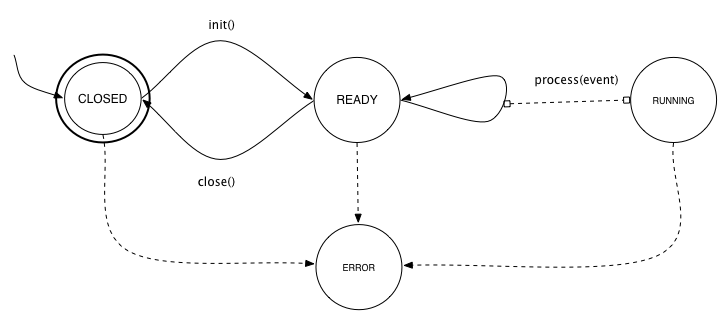
\includegraphics[width=\linewidth]{images/fsm-schema}
	\caption[\textit{EventProcessor} States Diagram]{The finite state machine diagram of any \name module and the Baselines. It is realised trough the \textit{Startable} interfaces, which provide the \textit{init()} and \textit{close() }methods, and trough the \textit{EventProcessor} interface, which declares the \textit{process(Event e)} method. The execution is possible only during the RUNNING state, which can be achieved by one and only module at time, as a constrain. The ERROR state prevents the propagation of erroneous behaviour to the data.}
  	\label{fig:module-fsm}
\end{figure}

The architecture of the \textsc{Test Stand} consists of three stand alone modules that establish a mono-directional communication flow: \textsc{Streamer}, \textsc{RSP Engine} and \textsc{Result Collector}. Moreover, the idea of an external structure which supports the other modules bring to the concept of the \textsc{Test Stand Supporting Structure}. All this components communicate exchanging events data, exploiting and event-based and modular architecture ad demanded by [R.10] and [R.11]. In the following we presents the two abstractions that allows this architecture: \textit{EventProcessor} and the \textit{Event}. Then we detail how the \textsc{Test Stand} Data Model is implemented.

\subsection{Abstractions}\label{sec:abstractions}

Among all the requirements reported in Section~\ref{sec:requirements} two of them are immediately relevant: [R.10], i.e. the need of an \textit{Extendible Design}, and [R.11], which states the necessity of an \textit{Event-base architecture} to properly face any RSPEngine. In order to to fulfil both \textsc{Test Stand} requires two main abstractions:
\begin{itemize}
\item The \textit{Event} - which is required to build a hierarchical communication. Indeed, the \textsc{Test Stand} may handle three events flows: one internal to the RSP Engine module, one for the communication between modules and one to communicate with the user. Next section about data clarifies the communication structured. 
\item The \textit{Event Processor} -  which guarantees the system to be modular, it standardizes the interaction simplifying the behaviour of each component in the system. Thus, a module is an \textit{Event Processor} which can be positioned everywhere in the the \textsc{Test Stand} pipeline
\end{itemize}

\noindent The requirement [R.4] directly influences the workflow of the \textsc{Test Stand}, quoting from Section~\ref{sec:requirements} \textit{The Test Stand must not be running when the RSP Engine is under execution}. 

To cover this requirement we designed the status of each module as a Finite State Machine (FSM), which can work only in those states that allow processing (READY). 

The schema in Figure~\ref{fig:module-fsm} represents the FSM that each module of \namens, the Baselines, and also for the \textsc{Test Stand External Structure} implements. 

The \textit{Startable} Interface standardises two methods, \textit{init()} and \textit{close()} which allow to control the behaviour of the module at the beginning and the end of the execution. The interface allows to move from the CLOSED state to the READY trough the \textit{init()} method and from the READY to the CLOSED trough the \textit{close()} method. 

The diagram is completed by the \textit{process (Event e)} method, which belongs to the \textit{EventProcessor} interface, The method brings the module into the RUNNING state until the processing ends, and then back to the READY one. As a constrain, one and only one module can be in the RUNNING state in a certain moment during the execution.

Finally, ERROR State, which can be reached from any point of the execution, prevents the propagation of errors over result data: when a module fails the execution is stopped without saving the erroneous data (last event) and reporting the error to the user.

Thus, each \name module implements the \textit{EventProcessor} and the \textit{Startable} interfaces in order to provide the behaviour presented in Figure~\ref{fig:module-fsm} by the FSM, fulfilling [R.10] and [R.11]. Moreover,  [R.4] is fulfilled since each module in the systems allows to be to explicitly controlled by the \textsc{Test Stand Supporting Structure}, which starts and stop the processing according to the RSP Engine execution status (see Section~\ref{sec:teststand}). 

\pagebreak

\subsection{Data Model}\label{sec:data-impl}

We already stated in the previous section that the \textsc{Test Stand} and its modules exploit an event-based communication, as required by [R.11]. Chapter~\ref{chap:heaven} describes \name workflow and how it exchanges events during the execution. Each event represent different data, depending on it position in the workflow. The \textit{Event} concept we introduced, which is implemented as an interface, allows to build the communication in many levels. In general \name handles four kinds of event, which are reported in Figure~\ref{fig:uml_events} and defined as follow:

\begin{figure}[h!tb]
  \centering
	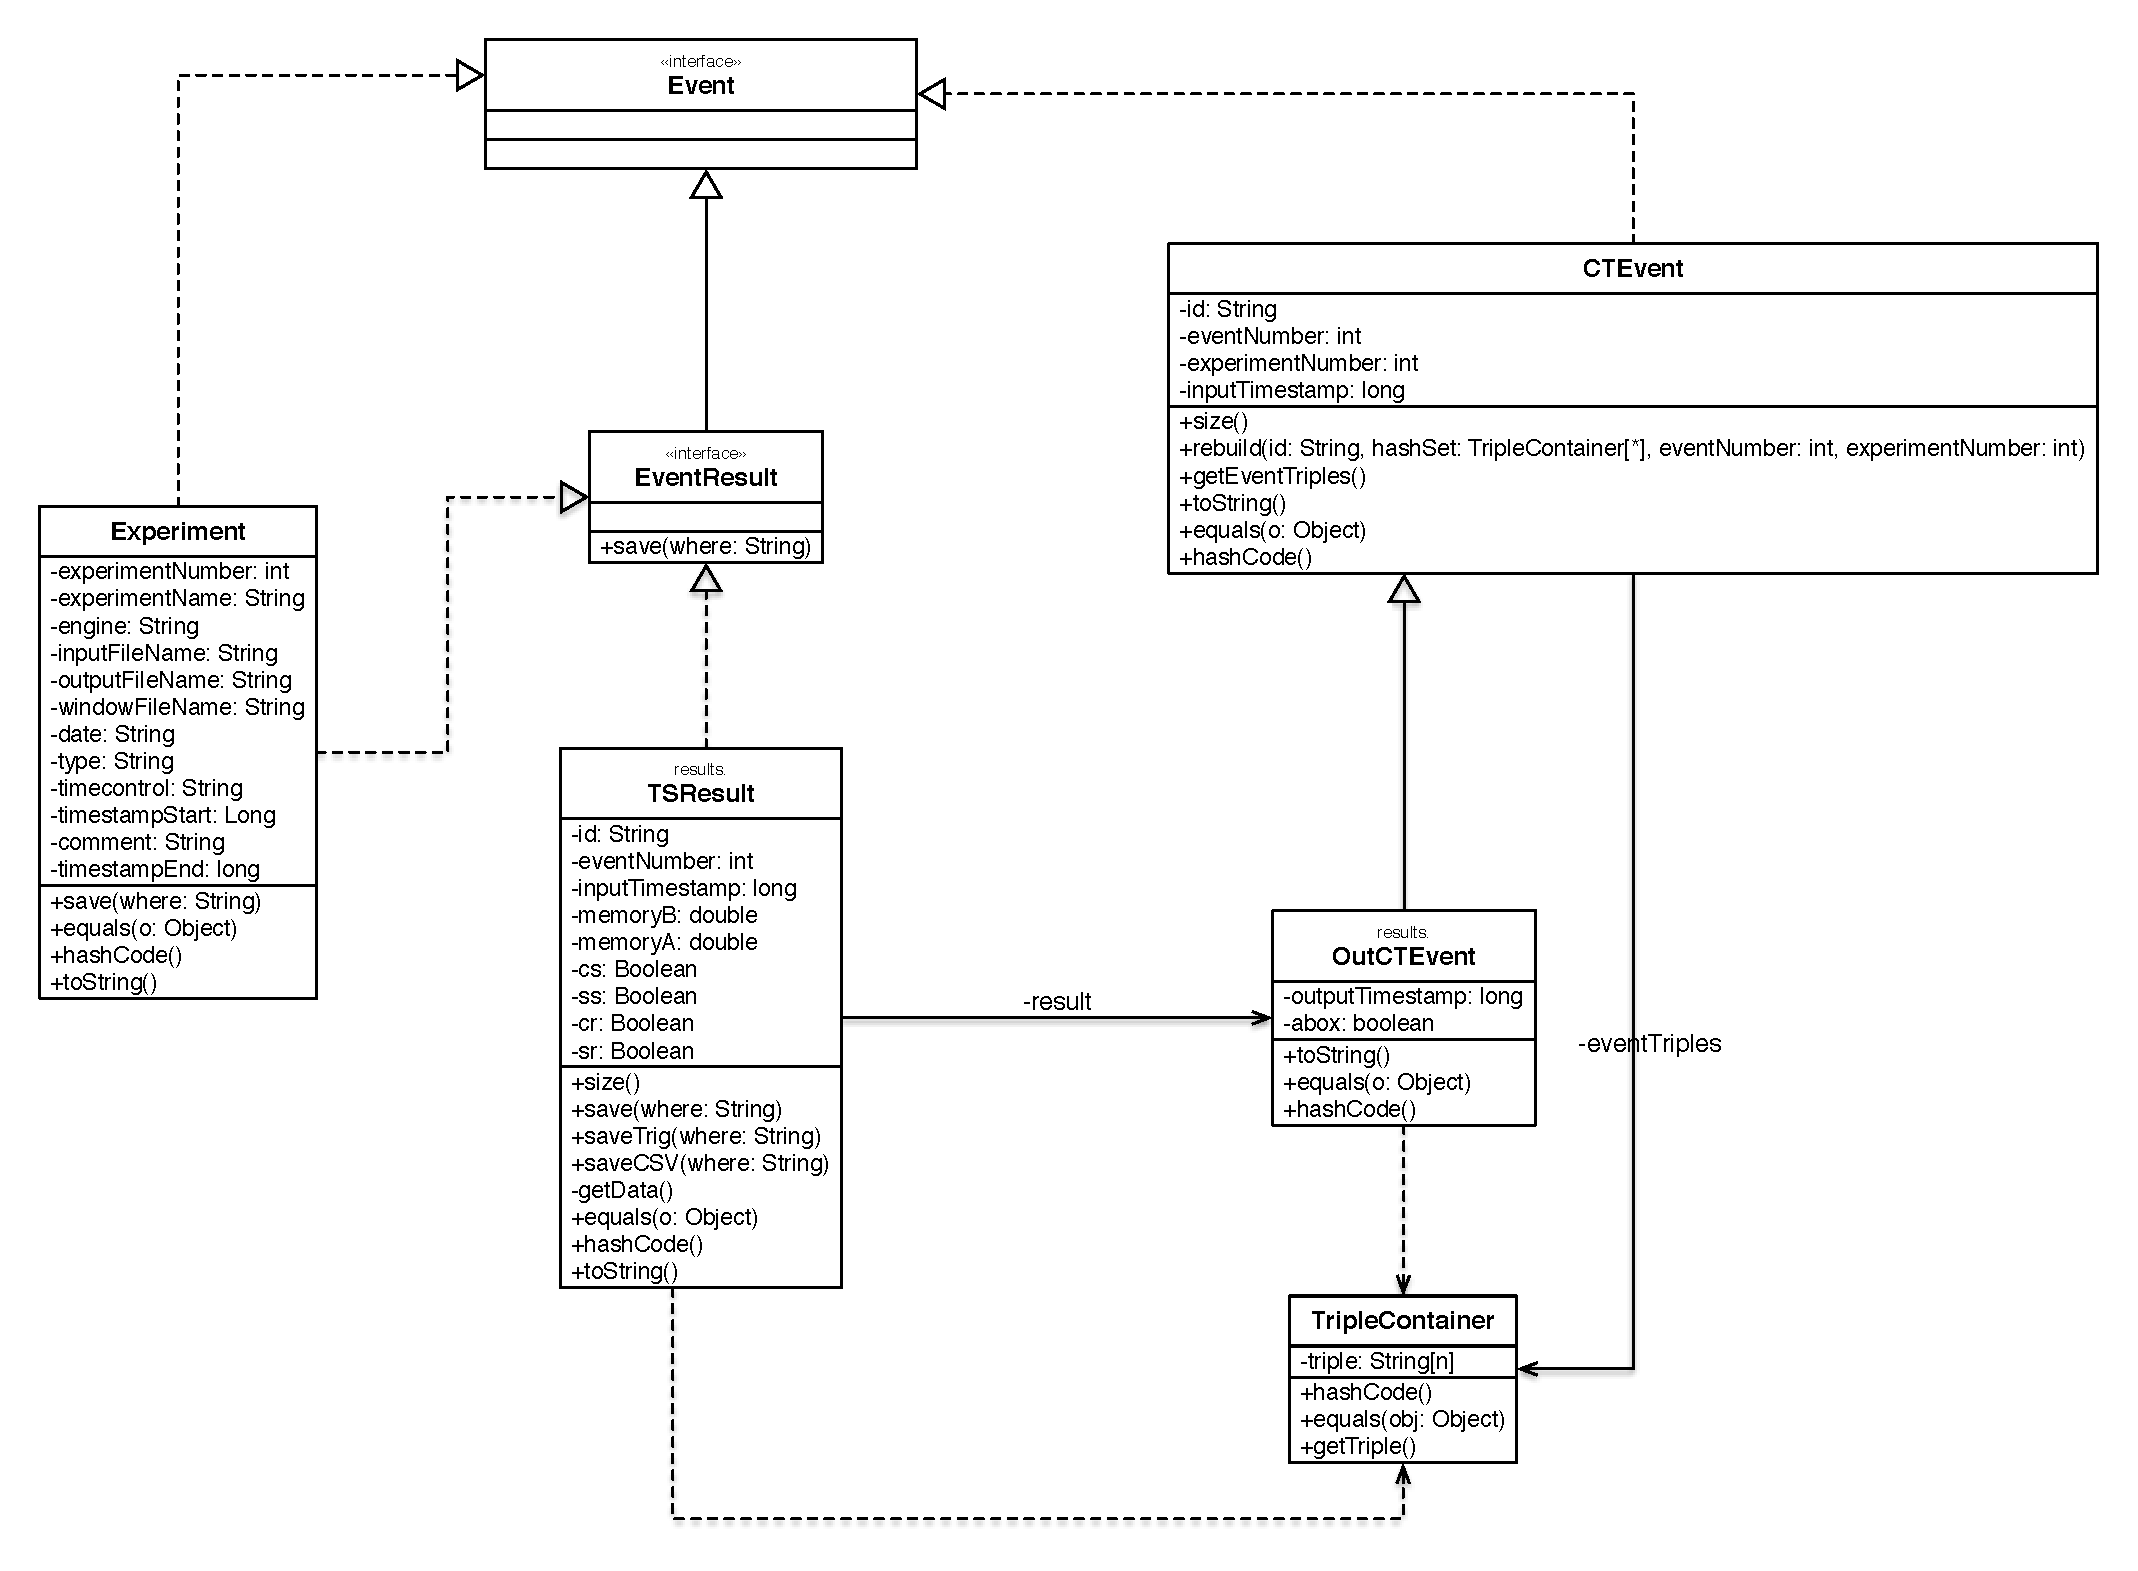
\includegraphics[width=\linewidth]{images/uml_events}
	\caption[\name Execution Events - UML Schema]{The figure shows the event that \name \textsc{Test Stand} and its modules 	exchanges during the execution of an experiment. All of them implement the \textit{Event} interfaces that start the class 	hierarchy.} 
	\label{fig:uml_events}
\end{figure}

\begin{itemize}
\item \textit{Experiment} - it represents the tuple $<\mathcal{E}, \mathcal{D},\mathcal{T},\mathcal{Q}>$, indicating which RSP Engine will be tested and with which queries, data and ontology will be used. It indicates if the current implementation of the engine exploit external timing. Finally the $type$ parameter indicates which kind of testing will be applied (SOAK o Stress for example) and it contains also the execution start time or end time.
\item \textit{CTEvent} - it contains a set of contemporary triples, wrapped in the \textit{TripleContainer}, which allows us to redefined hashcode and equals as a relation of the subject, object and predicate of the RDF triple. The id identifies the event within the experiment.
\item \textit{OutCTEvent} - it represents the event produced by the RSPEngine after processing the active window. Figure~\ref{fig:uml_events} show the inheritance relation between \textit{CTEvent}:  \textit{OutCTEvent} extends the \textit{CTEvent} adding the outputTimestamp field.
\item \textit{TSResult} - it wraps the \textit{OutCTEvent} adding the information about the minimal sensor data: memory, sampled ante e post processing, and latency. Two boolean fields allow complete and soundness result, if it is evaluated at runtime (see Section~\ref{sec:requirements})
\end{itemize}

\name requires an initialization phase to prepare and input the \textit{Experiment} into the \textsc{Test Stand}. The current implementation exploits a property file with the Experiment parameters: ID and the tuple $<\mathcal{E}, \mathcal{D},\mathcal{T},\mathcal{Q}>$. 

The \textit{CTEvent} and the \textit{OutCTEvent} contain RDF triples in NT-Triple\footnote{http://www.w3.org/2001/sw/RDFCore/ntriples/}, which is the easiest RDF serialisation to parse. This serialisation was chosen to fulfil requirement [R.12], which demands an \textit{Easy-to-Parse RDF Serialisation for the events presented to the RSP Engine in exam}. Figure~\ref{fig:uml_events} shows also that the RDF Triples are stored in the events into the \textit{TripleContainer} wrapper: we redefine the triple hashcode and equals method guaranteeing their uniqueness of within an \textit{CTEvent} or \textit{OutCTEvent}.

\section{Test Stand - Modules}\label{sec:modules-impl}

In this section we present the three modules which compose \namens, the \textsc{Streamer} and the \textsc{ResultCollector}, and also the \textsc{Test Stand Supporting Structure}. They all extend the \textit{EventProcessor} and the \textit{Startable} interfaces as reported in Section~\ref{sec:abstractions}.

In Section~\ref{sec:abstractions} we define a module as an \textit{EventProcessor} which can be positioned everywhere in the the \textsc{Test Stand} pipeline. We state that a module must implements the \textit{Startable} interface, which completes the FSM schema in Figure~\ref{fig:module-fsm} with the \textit{init()} and \textit{close()} methods.
Thus, each modules in this section offers three standard methods to interact with them: \textit{process(Event e)} from \textit{EventProcessor} and \textit{init()} and \textit{close()} from the \textit{Startable} Interface.

\subsection{Streamer}	\label{sec:streamer-impl}
\begin{figure}[tbh]
  \centering
	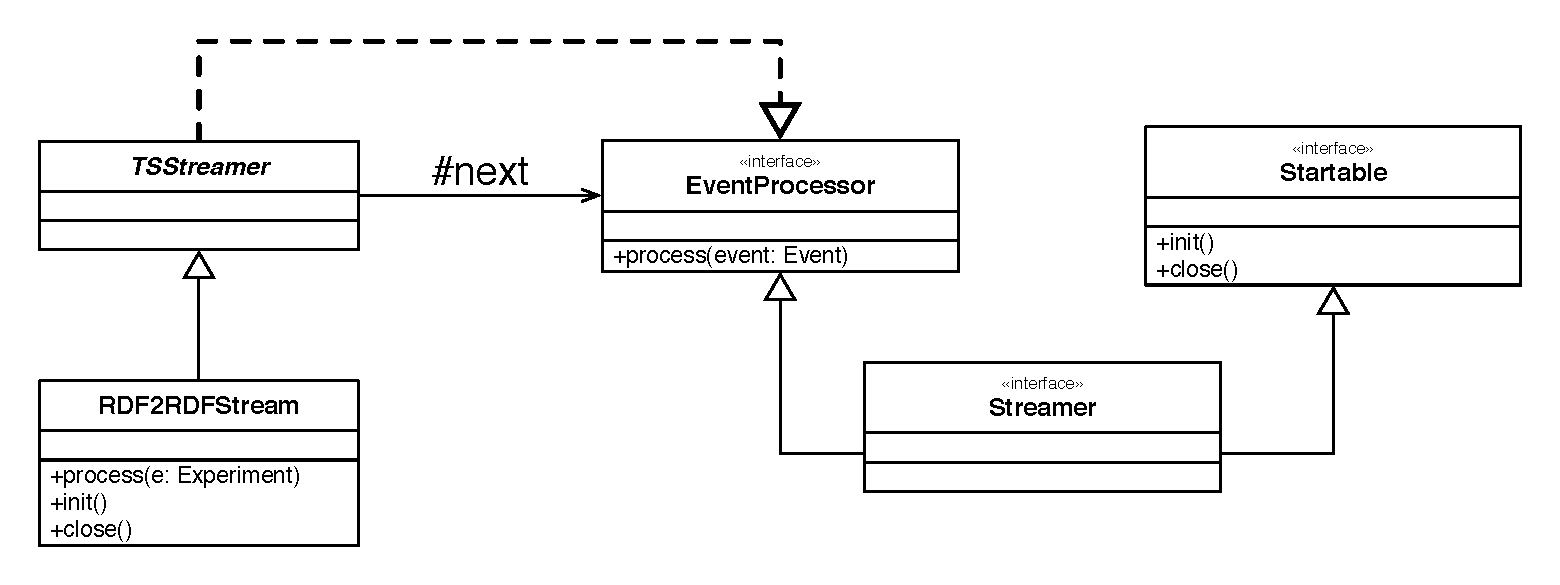
\includegraphics[width=\linewidth]{images/uml_tstreamer}
	\caption[\textit{RDF2RDFStream \textsc{Streamer} Implementation} - UML Schema]{Current implementation of the \textsc{Streamer} module. \textit{RDF2RDFStream} extends the \textit{TSStreamer} abstract class, which defines the module as an \textit{EventProcessor} of \textit{Experiment}s} 
  	\label{fig:uml_tstreamer}
\end{figure}

\noindent Figure~\ref{fig:uml_tstreamer} shows the current implementation of the \textit{Streamer} interface, which starts the \textsc{Test Stand} pipeline. Actually, the \textit{Streamer} is implemented as the \textit{TSStreamer} abstract class, which is specialised into processing of \textit{Experiment} events. 

The \textit{Experiment} events are  externally instantiated and then \textit{TSStreamer} receives them, and if initialised it can start the processining. It communicates with another \textit{EventProcessor}, called \textit{next} which can receive  \textit{CTEvent}s and it is represented in Figure~\ref{fig:uml_tstreamer} by the labelled arrow.  Notice that also the \textit{next} must be initialised before starting the communication, otherwise the ERROR state will be reached when the event is received by the \textit{next}, because the processing is not allowed.

Figure~\ref{fig:uml_tstreamer} contains also the \textit{RDF2RDFStream} implementation, whose internal structure can be seen in Figure~\ref{fig:uml_flowrateprofiler}. The \textit{RDF2RDFStream} was developed to conduct experiments as they are presented in Chapter~\ref{chap:evaluation}.  It is worth to note that we use LUBM Benchmarks to generate the data for the experiments. LUBM generated data are static, thus the \textit{RDF2RDFStream} builds an RDFStream attaching a timestamp to the static data produced by LUBM. %The file is generated using  LUBM(1000,0), which means 1000 different universities with the random generation seed 0. 

\begin{figure}[tbh]
  \centering
	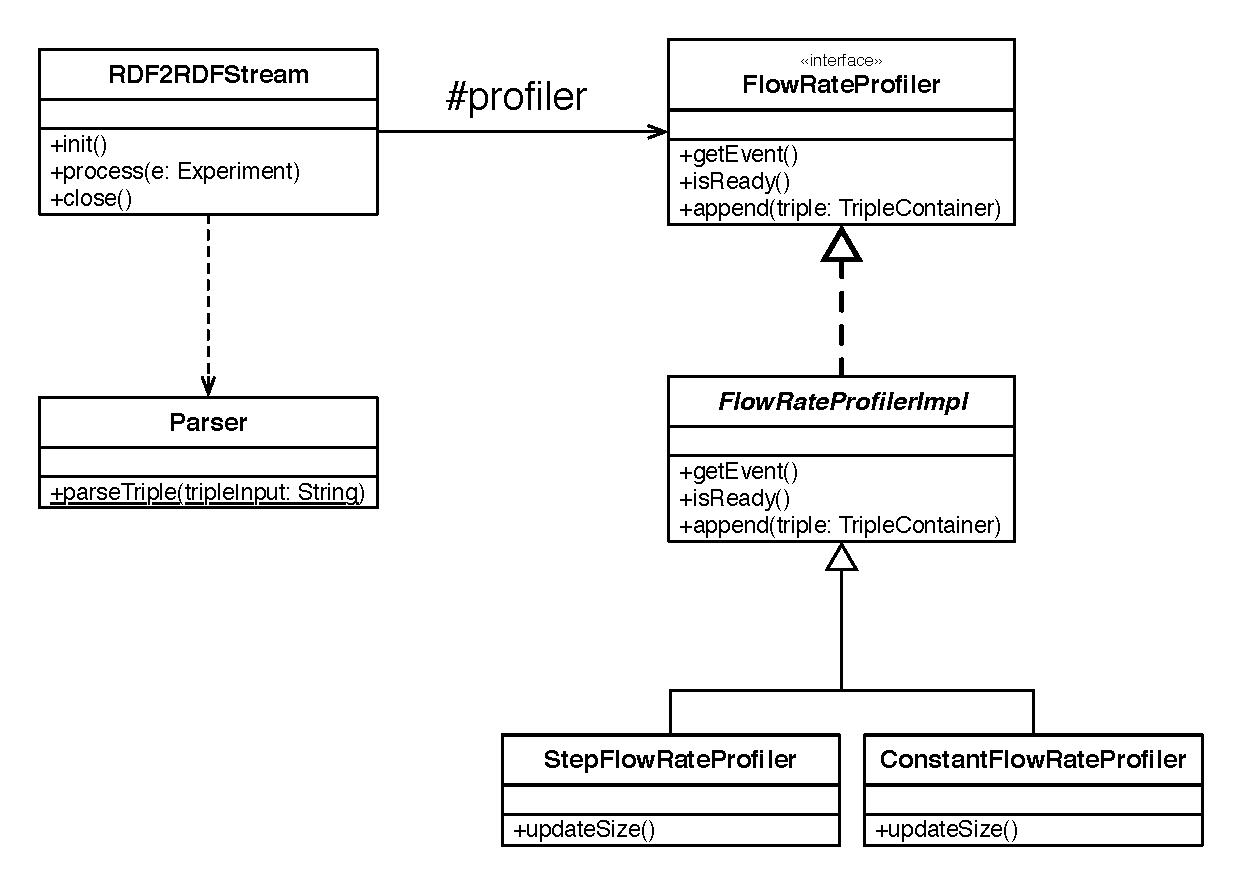
\includegraphics[width=0.75\linewidth]{images/uml_flowrateprofiler}
	\caption[Internal Components of \textit{RDF2RDFStream} - UML Schema]{The \textit{RDF2RDFStream} exploits two subcomponents to build an RDF Stream: the \textit{Parser}, which allows to ready in memory RDF Triples, and the \textit{FlowRateProfiler}, which attaches to RDF triple a timestamp and it builds \textit{CTEvent}s according to a function $f=f(x)$. The \textit{FlowRateProfileImpl} provides implementation of the \textit{append(TripleContainer tc}) method and of the two utility methods \textit{isReady()} and \textit{getEvent()}. Specific implementations of the \textit{FlowRateProfiler} control the function $f$ trough the \textit{updateSize()} method.} 
  	\label{fig:uml_flowrateprofiler}
\end{figure}


The \textit{Parser} component, in Figure~\ref{fig:uml_flowrateprofiler} can be accessed statically. It reads in memory one by one the triples in the file guaranteeing data independence [R.1] and it does not influence the memory footprint [R.5] by allocating only the memory necessary to parse a triple. 

Figure~\ref{fig:uml_flowrateprofiler} also includes the \textit{FlowRateProfiler}. This component determines the number of triples to add to a \textit{CTEvent} and it builds such an event. In this way, \textit{RDF2RDFStream} can generate different RDF streams to use as $\mathcal{D}$, which differ on the number of contemporary triples in the stream. 

\begin{figure}[tbh]
\centering
\subfigure[Exponential Growing \textsc{CTEvent} Size: $y=2^x$]{
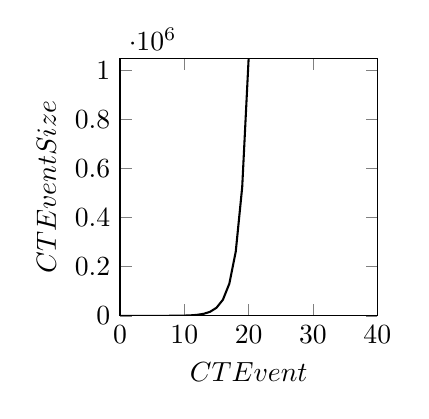
\begin{tikzpicture}
  \begin{axis}[ 
  width=0.4\linewidth,
      height=0.4\textwidth,
    xlabel=$CTEvent$,
    ylabel={$CTEvent Size$},
    xmin=0.00, xmax=40,
	ymin=0, ymax=1048576
  ] 
    \addplot [
    line width=0.75pt]
    coordinates {
    		(0.00, 1.00)
		(1.00, 2.00)
		(2.00, 4.00)
		(3.00, 8.00)
		(4.00, 16.00)
		(5.00, 32.00)
		(6.00, 64.00)
		(7.00, 128.00)
		(8.00, 256.00)
		(9.00, 512.00)
		(10.00, 1024.00)
		(11.00, 2048.00)
		(12.00, 4096.00)
		(13.00, 8192.00)
		(14.00, 16384.00)
		(15.00, 32768.00)
		(16.00, 65536.00)
		(17.00, 131072.00)
		(18.00, 262144.00)
		(19.00, 524288.00)
		(20.00, 1048576.00)
		};	
		
	\end{axis}
\normalsize

\end{tikzpicture}
}
\subfigure[Step Growing Size with K1=100 and K2=1000 after 9 \textsc{CTEvents}]{
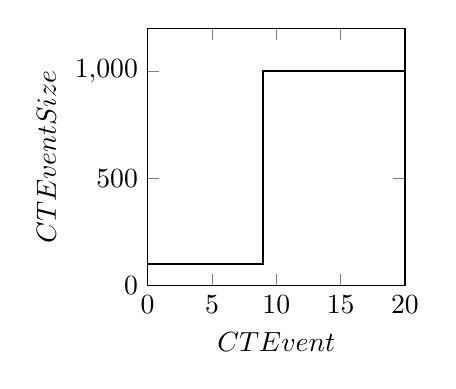
\begin{tikzpicture}
  \begin{axis}[ 
  width=0.4\linewidth,
      height=0.4\textwidth,
    xlabel=$CTEvent$,
    ylabel={$CTEvent Size$},
    xmin=0.00, xmax=20,
	ymin=0, ymax=1200
  ] 
    \addplot [
    line width=0.75pt]
    coordinates {
    		(0.00, 100.00)
		(1.00, 100.00)
		(2.00, 100.00)
		(3.00, 100.00)
		(4.00, 100.00)
		(5.00, 100.00)
		(6.00, 100.00)
		(7.00, 100.00)
		(8.00, 100.00)
		(9.00, 100.00)
		(9.00, 1000.00)
		(10.00, 1000.00)
		(11.00, 1000.00)
		(12.00, 1000.00)
		(13.00, 1000.00)
		(14.00, 1000.00)
		(15.00, 1000.00)
		(16.00, 1000.00)
		(17.00, 1000.00)
		(18.00, 1000.00)
		(19.00, 1000.00)
		(20.00, 1000.00)
		};	
		
	\end{axis}
\normalsize

\end{tikzpicture}
}
\caption[Example of FlowRateProfiler Triple Distribution]{The \textsc{FlowRateProfiler} is able to calculate \textsc{CTEvent} size according to a function which relates the number of triple to the number of \textsc{CTEvent} }
\label{fig:frp-examples}
\end{figure}


The \textit{FlowRateProfilerImpl} implements \textit{FlowRateProfiler} interface. It provides a common implementation for the method \textit{append(TripleContainer tc)}, which adds to the current \textit{CTEvent} an RDF triple,  and of the two utility methods \textit{isReady()} and \textit{getEvent()}. What variates between different implementations of this component, is the \textit{updateSize()} method. 

The \textit{FlowRateProfiler} creates \textit{CTEvent} according to a function $y=f(x)$, in which $x$ is the number of the \textit{CTEvent} and it results that $y$ is the number of triple this \textit{CTEvent} will contain. The update logic given by $f$ is implemented within the \textit{updateSize()} method. For example if we decide to increase linearly the number of triples inside a \textit{CTEvent} the function $f$ will be: \[y=x, \text{ where } x,y \in N\]
The first event (E0) will contain zero triple, E1 will contain only one triple following E4 will contain four triples and so forth. Another possibility is to increase exponentially the number of triples inside a \textit{CTEvent} : \[y=2^x, \text{ where } x,y \in N\]The first event (E0) will contain one triple, E1 will contain two triple following E3 will contain eight triples and so forth, Figure~\ref{fig:frp-examples}.a shows the resulting behaviour plotting the triple number on y-axis and \textit{CTEvent} number on x-axis.



In the current stage of development we include four implementations of the \textit{FlowRateProfiler}, two of them are related to our experiments: 
\begin{itemize}
\item \textit{ConstantFlowRateProfiler} - it maintains the same number of triples for each events over all the experiment: \\
\[y=K, \text{ where } K \in N \]

\item \textit{StepFlowRateProfiler} - it maintains a constant number of triple $K1$ inside a \textit{CTEvents} for $x$ occurrences, then it suddenly changes the number of triple $y$ form $K1$ to $K2$ where $K2 >> K1$. The number of  \textit{CTEvents} $x$ is specified in the set-up phase of the component.  Figure~\ref{fig:frp-examples}.b contains the resulting plot of implemented function which follows:

\[
y=
\begin{cases}
K1, &\text{if $x < M$ } $ where $ K1, M \in N\\
K2, &\text{if $x >= M$} $ where $ K2 >> K1, K2 \in N
\end{cases}
\]


\end{itemize}

The remaining two  \textit{FlowRateProfiler} implementations in \name that are not related to our evaluation are:
\begin{itemize}
\item \textit{LinearStepFlowRateProfile} - it streams $x$ \textsc{CTEvents} of dimension $y$, in terms of triples, then linearly increase the number of a quantity $M$: \[y=x*M, \text{ where } x,y,M \in N\]
\item \textit{ConstantRandomFlowRateProfiler} - it changes $y$ and $x$ according with two random integer generators directed by two seeds. The generators provided integer numbers according to a certain probability \[y=randomInt(seed), \text{ where } random(seed),y \in N\]
\end{itemize}


\subsection{Result Collector} 

\noindent The \textsc{ResultCollector} is the data acquisition system that receives and persist the query results and the measurements data gathered by the \textsc{Test Stand} during the execution of an experiment.

\begin{figure}[tbh]
  \centering
	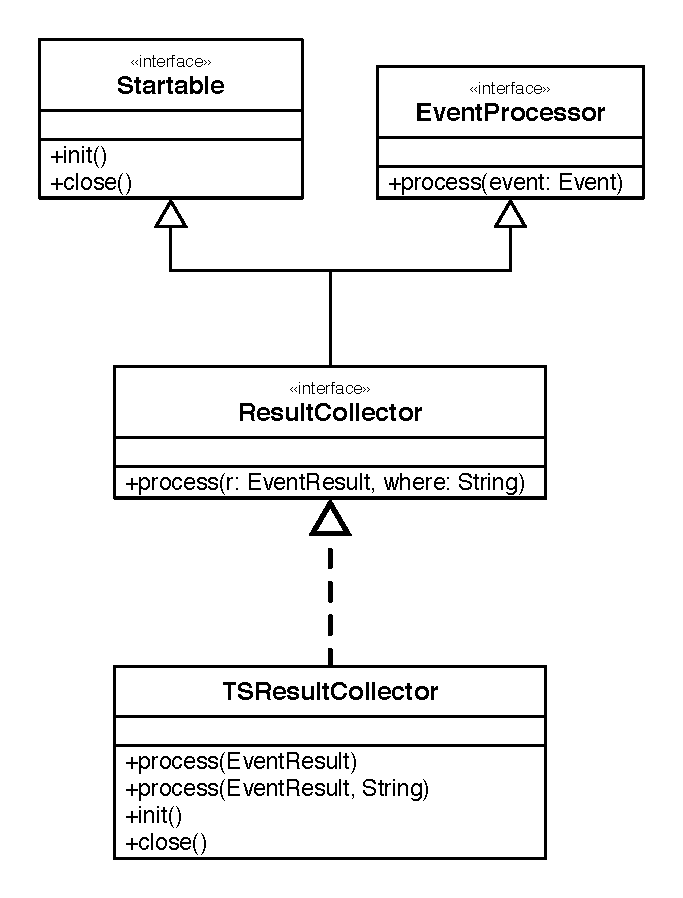
\includegraphics[width=0.5\linewidth]{images/uml_resultcollector}
	\caption[\textsc{ResultCollector} Current Implementation - UML Schema]{The current implementation of the \textsc{ResultCollector} interface is the \textit{TSResultCollector} which processes events that implements the \textit{EventResult Interface}. \textit{ResultEvent} interface hides the saving procedure, delegating the implementation to the event provider trough    the \textit{save()} method. \textit{TSResultCollector} exposes also the method process(Event e, String where), which allows the caller to specify the destination. } 
  	\label{fig:uml_resultcollector}
\end{figure}

The UML Schema in Figure~\ref{fig:uml_resultcollector} shows firstly that the \textit{ResultCollector} interface is again an extension of the \textit{EventProcessor} and the \textit{Startable} ones. The current implementation is the \textit{TSResultCollector}, which stays at the end position in the \textsc{Test Stand} pipeline. The \textit{ResultCollector} is responsible of saving data in a way that is independent from which data format, since requirement [R.7] demands to \textit{enable users extensions with new software sensors and specific measurements collection}. The \textit{TSResultCollector} applies a general saving procedure exploiting the \textit{EventResult} interface, which exposes the \textit{save(String where)} method to delegate the implementation of such a procedure to the provider of the event. Figure~\ref{fig:uml_resultcollector} shows the relation between the \textit{EventResult} interface and the \textit{TSResultCollector}, which specialises the processing method to \textit{process(EventResult} and it known the general destination of the data, but it also exposes a secondary one \textit{process(EventResult, String where)}, which allows the caller to specify the saving path.


\begin{figure}[tbh]
  \centering
	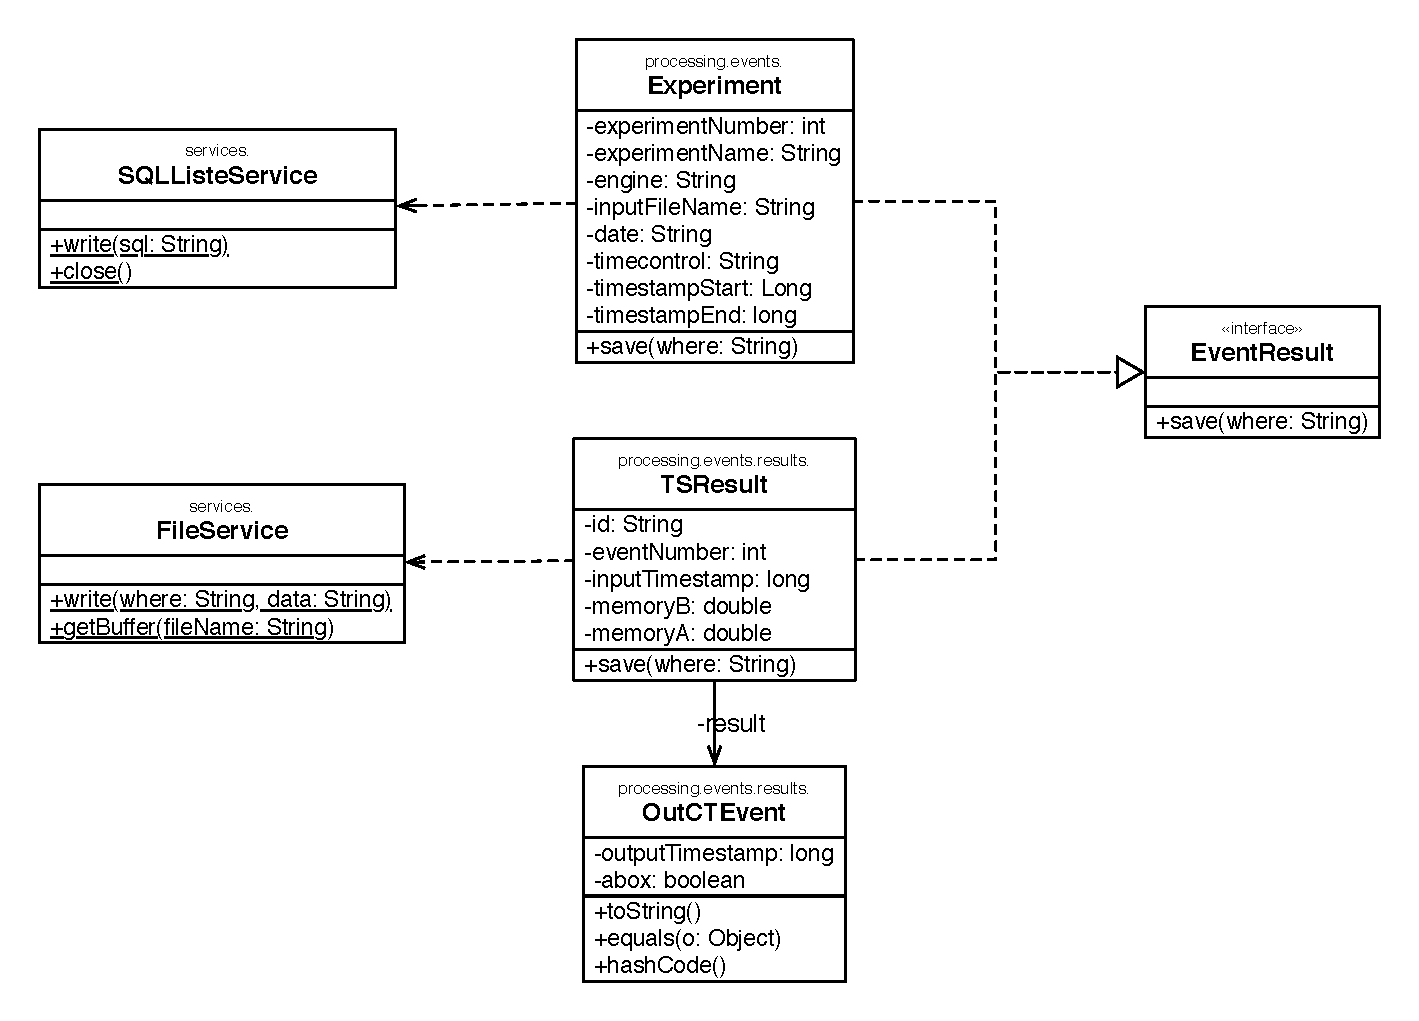
\includegraphics[width=\linewidth]{images/uml_resultcollector_events}
	\caption[\textsc{ResultCollector} Events - UML Schema]{ All the \textit{Experiment}, the \textit{TSResult} and the \textit{OutCTEvent} implements the \textit{EventResult} interface in order to hides specific saving procedure behind the \textit{save(String where)} method. The saving procedures exploits two service classes the \textit{FileService} and the \textit{SQLLIsteService}, which avoid concurrent access to the saving procedure with static methods.} 
  	\label{fig:uml_resultcollector_events}
\end{figure}

Figure~\ref{fig:uml_resultcollector_events}, shows how different events in the system exploit the \textit{EventResult} interface. In the current implementation the \textit{TSResultCollector} handles two kinds of event:
\begin{itemize}
\item \textit{TSResult} - it saves the data of the query results into a TriG\footnote{http://www.w3.org/TR/trig/} file where the graph name is the event id inside the experiment, while it saves the measurements data into a CSV\footnote{$http://en.wikipedia.org/wiki/Comma-separated_values$} file that represent the time series w.r.t events id. 
\item \textit{Experiment} - it saves the experiment metadata and the tuple \\ $<\mathcal{E},\mathcal{D},\mathcal{T},\mathcal{Q}>$ collapsed into a generic description field into SQLite\footnote{https://sqlite.org/} database.
\end{itemize} 

Both the saving procedure exploit a service class, respectively the \textit{FileService} and the \textit{SQLLIsteService}. In Figure~\ref{fig:uml_resultcollector_events} are describe those services, which expose static methods to interact with the file-system. The goal is reducing system complexity offering a single point of interaction with the file-system. In this way is possible  to avoid parallel interactions that may influence the experiment. 


\subsection{Test Stand Supporting Structure}\label{sec:teststand-impl}


\begin{figure}[tbh]
  \centering
	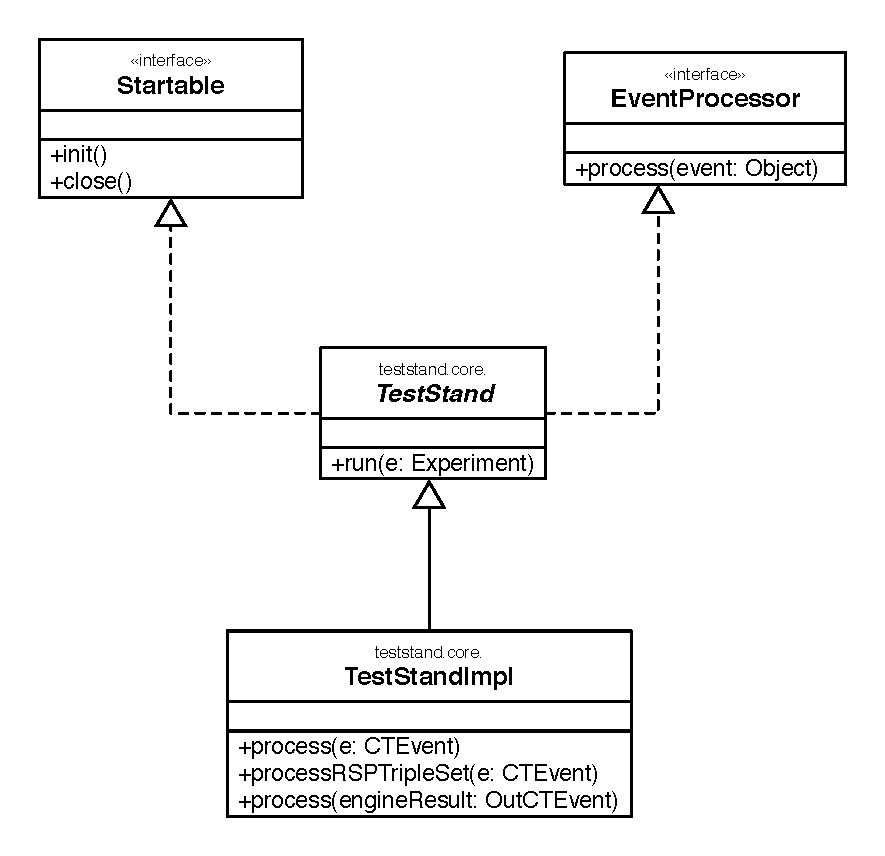
\includegraphics[width=0.5\linewidth]{images/uml_teststand}
	\caption[\name \textsc{TestStand} - UML Schema]{The \textsc{TestStand} abstract class implements both the \textit{EventProcessor} and the \textit{Startable} interfaces, but defines only the methods \textit{init()} and \textit{close()}  and it adds the \textit{run(Experiment e)} method, which encapsulate the execution logic. The \textit{process(CTEvent e)} method is implemented by \textit{TestStandImpl} which represents the \textit{Test Stand External Structure}. It orchestrates the communication between other modules and gather the data.}
  	\label{fig:uml_teststand}
\end{figure}


\noindent \name \textsc{Test Stand} was defined as set of modules which interact exchanging events during the execution. However, Chapter~\ref{chap:heaven} describes at the design level the presence of an external structure which orchestrates the communication between the \textsc{Streamer}, the \textsc{RSP Engine} and the \textsc{ResultCollector}. This external structure also exposes the APIs for users interaction. Figure~\ref{fig:uml_teststand} represent this idea into an UML schema where the abstract class \textit{TestStand} implements both the \textit{Startable} interface  defining the \textit{init()} and \textit{close()} methods and also the \textit{EventProcessor} interface, but it leaves the implementation of the \textit{process(CTEvent e)} method to the current implementation: the \textit{TestStandImpl}. 

The relation between the \textit{TestStand} and other modules is presented in Figure~\ref{fig:uml_teststand_modules}. The \textit{TSStreamer}, the \textit{RSPEngine} and the \textit{TSResulCollector} are linked to the \textit{TestStandImpl} trough an initialisation class which receives the configuration file, and sets up these modules according with the requirements [R.1]  [R.2] and [R.3] (respectively data independence, engine independence and query independence). Once the set-up phase is completed the \textit{TestStandImpl} is initialized and it consequently initialises all the upstanding modules. The \textit{Experiment} is created externally and  the \textit{TestStandImpl} receives it to start the execution. 

During the execution \textit{TestStandImpl} gets the \textit{CTEvents} form the \textit{TSStreamer} and sends them to the \textit{RSPEngine} (see Section~\ref{sec:test-stand-workflow}). The \textit{TestStandImpl} gathers the measurements data according with the \textit{Experiment} specification. It calculates latency starting a timer when the \textit{CTEvent} arrives and stopping the timer when it \textit{RSPEngine} outputs the results as \textit{OutCTEvent}. It retrieves the memory usage asking the JVM in both the point above [R.6]. To fulfil requirements [R.7] any new measurement can take place only when the \textit{RSPEngine} is not running. Once the \textit{OutCTEvents} comes form the \textit{RSPEngine}, the \textit{TestStandImpl} immediately wraps the event into a \textit{TSResult}, which is sent to the \textit{TSResultCollector} to persist the query results and the measurement data, fulfilling [R.8] and supporting [R.9] for further analysis with the \textsc{Analyser}.

\begin{figure}[p!]
  \centering
	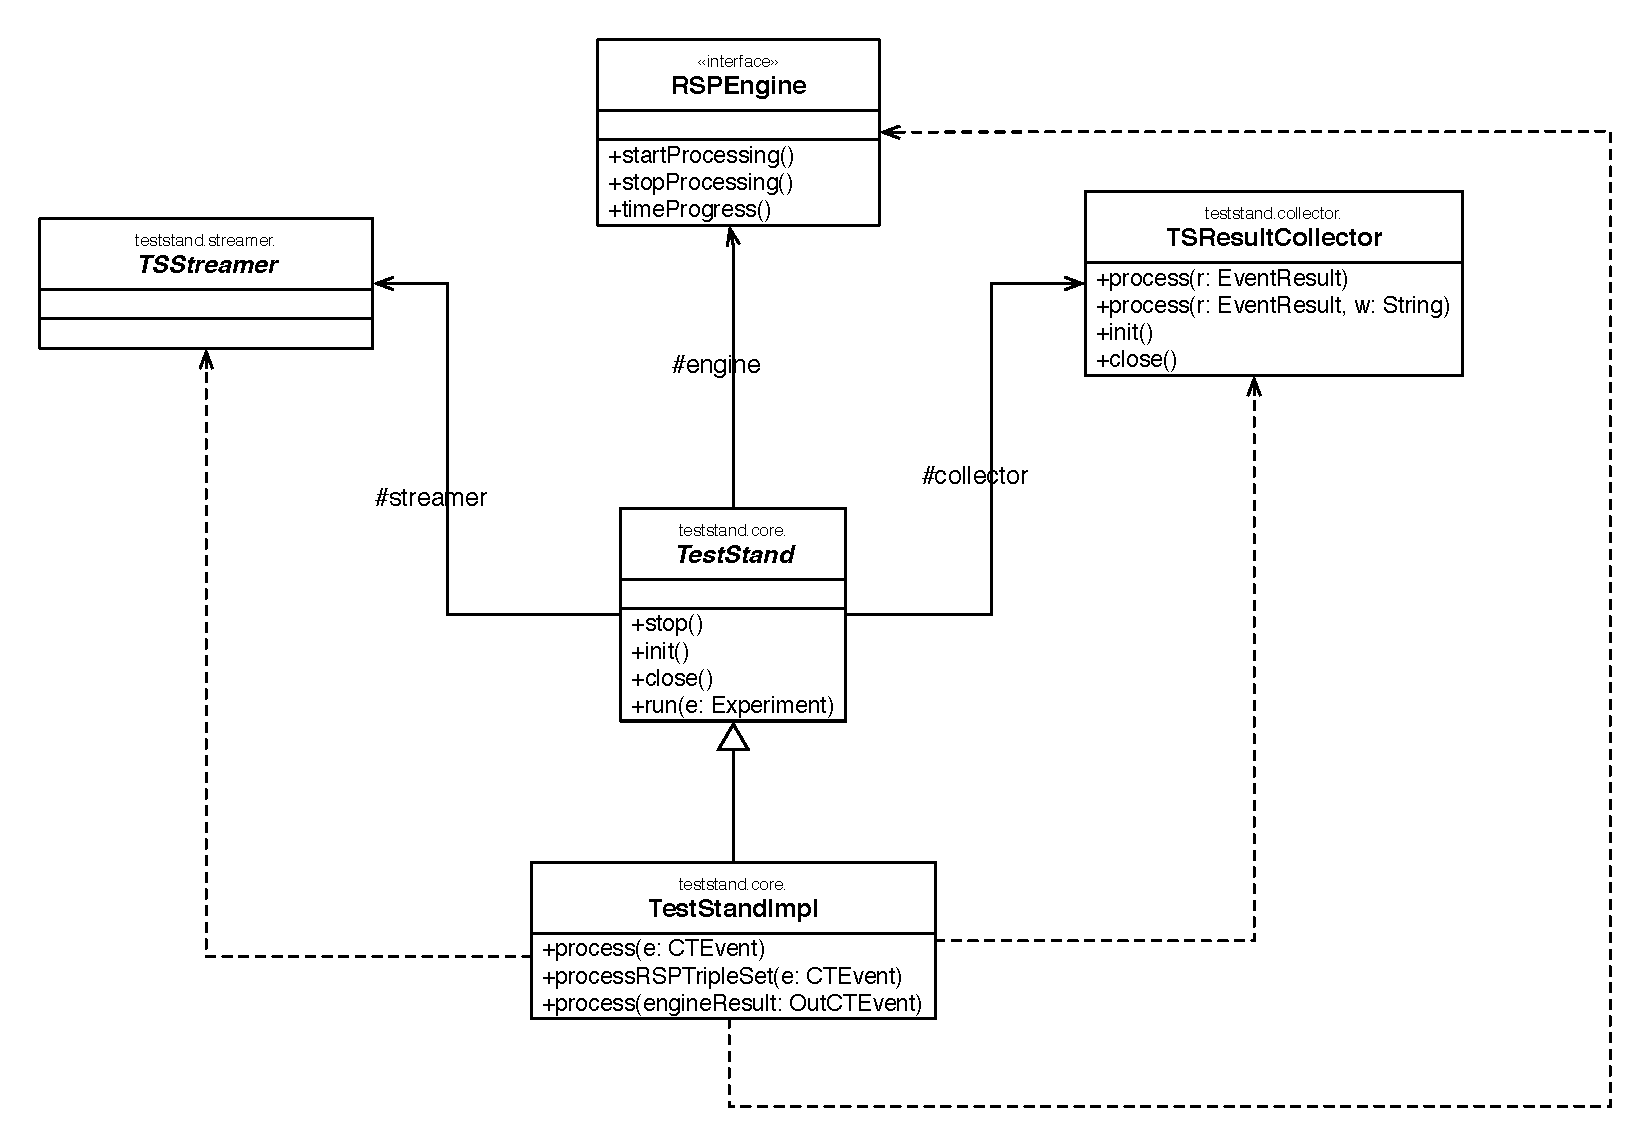
\includegraphics[width=0.9\linewidth]{images/uml_teststand_modules}
	\caption[\name \textsc{TestStand} and Modules  - UML Schema] {The \textit{TestStand} contains references of the \textit{TSStreamer}, the engine behind the \textit{RSPEngine} interface and the \textit{TSResultCollector}. The \textit{TSStreamer} and current \textit{RSPEngine} are linked to the next element in the pipeline trough the \textit{TestStand}. Two arrows, labelled with "next", point to the  \textit{TestStand} indicating that it receives the events from all modules and it orchestrates the communication. The arrow which start from the \textit{RSPEngine} is coloured in gray to highlight that it can not be seen at this level of detail, because \textit{RSPEngine} is an interface. The \textit{ResultCollector} receives the result to save at the end of each cycle, it does need a "next", because the process ends when it returns the call.} 
  	\label{fig:uml_teststand_modules}
\end{figure}

\pagebreak

\section{Baselines}\label{sec:baselines-impl}

\name Baselines are four elementary implementations of an RSP Engine, which  cover the requirements form [R.13] to [R.16] and implement the pipeline of a DSMS with a reasoner following the proposal presented in Section~\ref{sec:baselines}. 
The RSP Engine pipeline is composed by Esper\footnote{$http://www.espertech.com/esper/$}, a mature commercial DSMS, with the Jena general purpose rule engine\footnote{http://jena.apache.org/documentation/inference/\#rules}, a flexible reasoning engine.  The aim of the choice of Esper and Jena is fulfilling requirement [R.14], baselines Eligibility by coupling two mature solutions for stream processing and reasoning to obtain a fair solution in the SR context.

\begin{figure}[tbh]
  \centering
	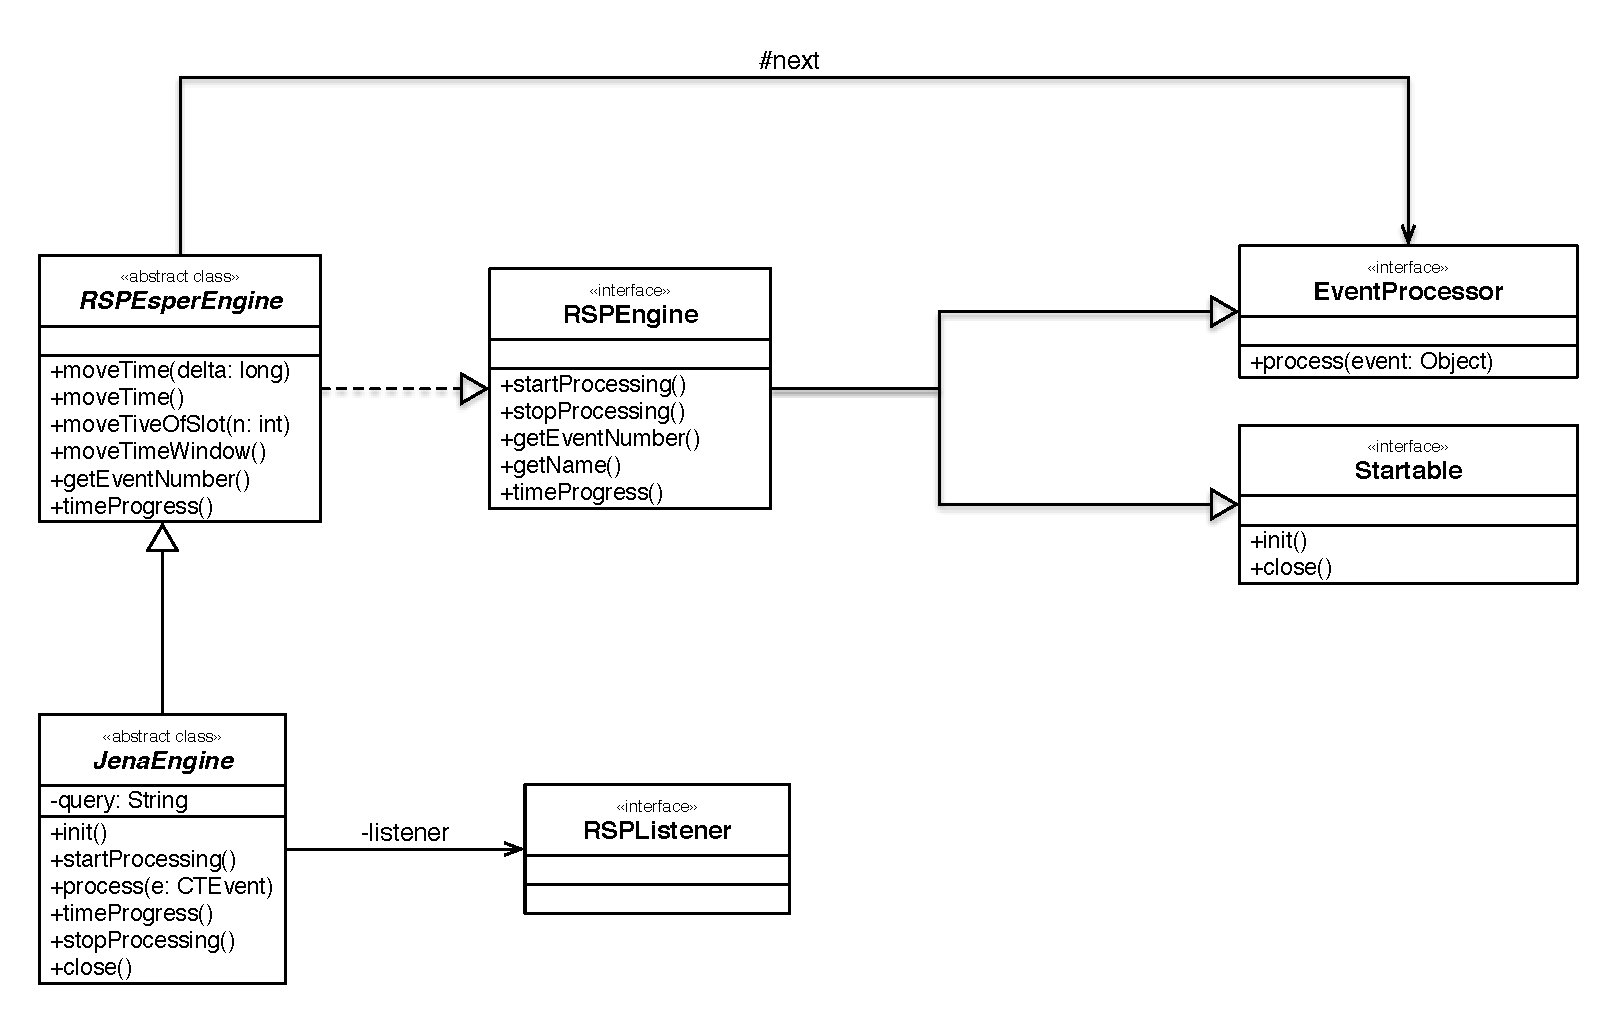
\includegraphics[width=\linewidth]{images/uml_baselines_general}
	\caption[\textit{RSPEngine} Implementation Trough Esper and Jena - UML Schema]{The \textit{RSPEngine} interface extends both the \textit{EventProcessor} and the \textit{Startable} ones. The \textit{RSPEsperEngine} class in picture implements the interface adding the Esper runtime to handle its internal events. The \textit{JenaEngine} together with the \textit{RSPListener} integrate the Jena reasoning system into the engine.}
  	\label{fig:uml_baselines_general}
\end{figure}

\noindent Figure~\ref{fig:uml_baselines_general} presents how the baselines are implemented. The general structure exploits the \textit{RSPEngine} interface, a proxy for both the \textit{EventProcessor} and the \textit{Startable} interfaces described in  in Section~\ref{sec:abstractions}. 

\name Baselines integrate Esper as the DSMS which compose the first half to the RSP Engine pipeline.  The \textit{RSPEsperEngine} abstract class implements the \textit{RSPEngine} interface in order to share the Esper runtime definition for all the Baselines.  They exploit the ability of Esper to be temporally controlled by an external agent\footnote{\url{http://esper.sourceforge.net/esper-0.7.5/doc/reference/en/html_single/index.html#api-controlling-time}}. Thus, the internal time flow can be synchronised by sending time-keeping events. In this way it possible to ensure the complete and soundness of query results, even in case of high traffic load. To enable external time control the \textit{RSPEngine} interface exposes the \textit{moveTime()} method.  The \textit{RSPEsperEngine} implements \textit{moveTime()} encapsulating the logic to send a time-keeping event into Esper: one time-keeping event is sent before injecting the triples within a \textsc{CTEvent} and the next one after all triples in \textsc{CTEvent} were sent. In this way all the triples in the \textsc{CTEvent} are consider contemporary by the Baselines. 

The RSP Engine is in the middle of the \textsc{Test Stand} pipeline, thus is has to communicate with the module below. The \textit{RSPEsperEngine} has a reference to a general \textit{EventProcessor}, represented in Figure~\ref{fig:uml_baselines_general}  by the arrow labeled as "next", which can be any modules which processes \textit{CTEvent}. In the current implementation the \textsc{Test Stand External Structure}, implemented as the \textit{TestStandImpl} class, follows \textit{RSP Engine}, to intercept the outcoming\textit{OUTCTEvents}.

\begin{figure}[tbh]
  \centering
	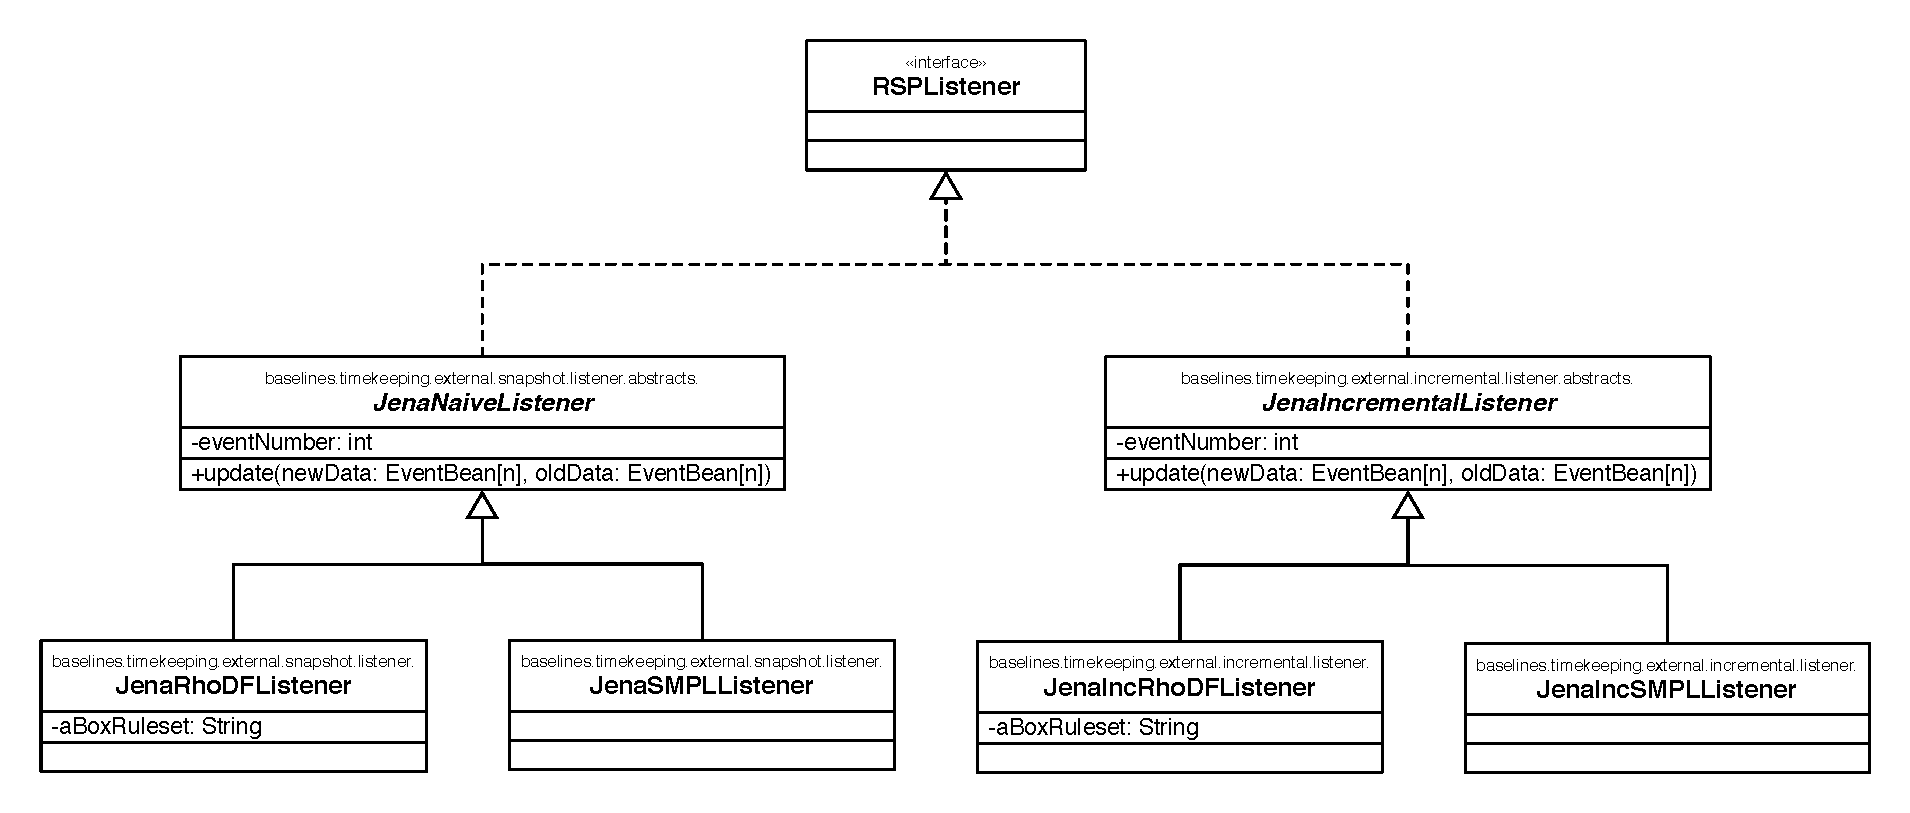
\includegraphics[width=\linewidth]{images/uml_baselines_listener}
	\caption[\textit{RSPListener} Implementations - UML Schema]{The \textit{RSPListener} is actually a proxy for the native Esper \textit{UpdateListener}. We implement the interface following two possible reasoning approaches, Naive and Incremental, respectively into the  \textit{JenaNaiveListener} and the \textit{JenaIncrementalListener}. Further implementations like the \textit{JenaNaive$\rho$DFListener} allows to specify the entailment regime and the TBox to the listeners.} 
  	\label{fig:uml_baselines_listener}
\end{figure}

We draw in Figure~\ref{fig:uml_baselines_general} the UML schema of the Baseline implementation. The \textit{JenaEngine} abstract link the DSMS to the reasoner, an thus it requires a further component, the RSPListener, to complete the RSP Engine pipeline and realise the system we describe in Section~\ref{sec:baselines}
 
The reasoner stage is realised as shown in Figure~\ref{fig:uml_baselines_listener}. Different implementations of the listener, which all belongs to the the \textit{RSPListener} interface, variate the reasoning approaches between Naive or Incremental. The \textit{JenaNaiveListener} or the \textit{JenaIncrementalListener} partially fulfil requirement [R.15] (baseline relevance) in terms of reasoning. None of the two specify the entailment regime and the TBox, which must be defined with specific implementations like the \textit{JenaRHODFNaiveListener}, as it is visible again in the Figure~\ref{fig:uml_baselines_listener}.

\begin{figure}[p!]
  \centering
	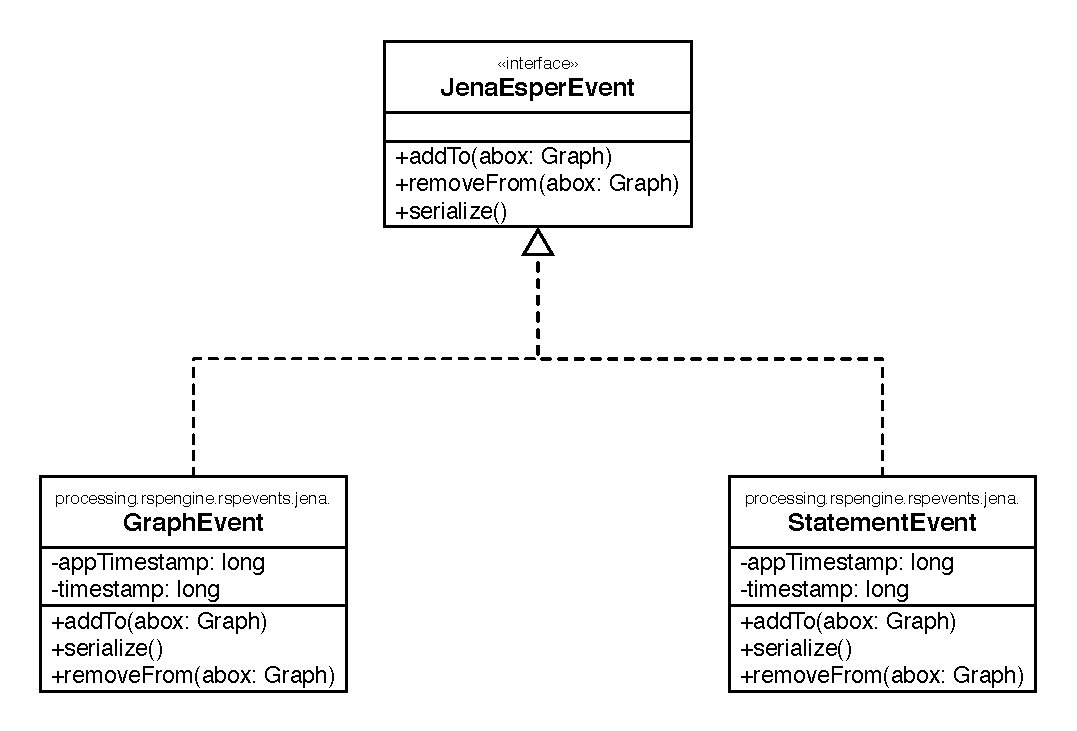
\includegraphics[width=0.8\linewidth]{images/uml_baselines_events}
	\caption[Esper-level Graph based and Triple based - UML Schema]{ All the event registered to Esper belong to the \textit{JenaEsperEvent} interface, which exposes methods to handle the reasoning independently from the RDF Stream implementation:  \textit{GraphEvent} or \textit{TripleEvent}. The triples received by the \textit{RSPEngine} can be pushed into Esper as complete graph or as a set statements. To handle the active window graph independently from the event implementation, the interface exposes the method \textit{addTo(Graph g)} and \textit{removeFrom(Graph g)}, while the \textit{serialise()} methods unroll the current event into a set of statement, in order to build an outgoing \textit{OutCTEvent}}
  	\label{fig:uml_baselines_events}
\end{figure}

The Baselines relevance demanded by [R.15] it is only partially fulfilled by the alternative reasoning approaches. It comes also from the different implementation of the RDFStream model, graph based or triple based. Esper runtime demands to registers the events that it has to handle. Figure~\ref{fig:uml_baselines_events} shows how events are implemented: they belongs to the e \textit{JenaEsperEvent} interface, which exposes three methods used by the \textit{RSPListener} to manage the active window independently from event implementation. The methods \textit{addTo(Graph g)} and \textit{removeFrom(Graph g)} adelegates to the event the operations of insert and deletion to the event, in a transparent way for the \textit{RSPListener}; the method \textit{serialise()} unrolls the event into a set of statements, in this way the RSP Engine can output an \textit{OutCTEvent} independently from the RDF Stream implementation: \textit{GraphEvent} or \textit{TripleEvent}

Notice that when a \textit{CTEvents} comes to the RSP Engine it will be transformed into the events handled by the DSMS, contained in Figure~\ref{fig:uml_baselines_events}. This translation process influences the latency calculus, because the time spent by the engine to translate events from the RDFStream into its internal mechanism may be relevant. Once the processing is complete, the output of the RSP Engine is translated again into an \textit{OutCTEvent} and passed to the next \textit{EventProcessor}, again spending time that influence the latency.

The current Baselines implementation divides the different architectural elements and delegates to each element a specific task to share the majority of the code and thus fulfilling [R.16], which demands baseline Simplicity.

%\begin{figure}[tbh]
%  \centering
%	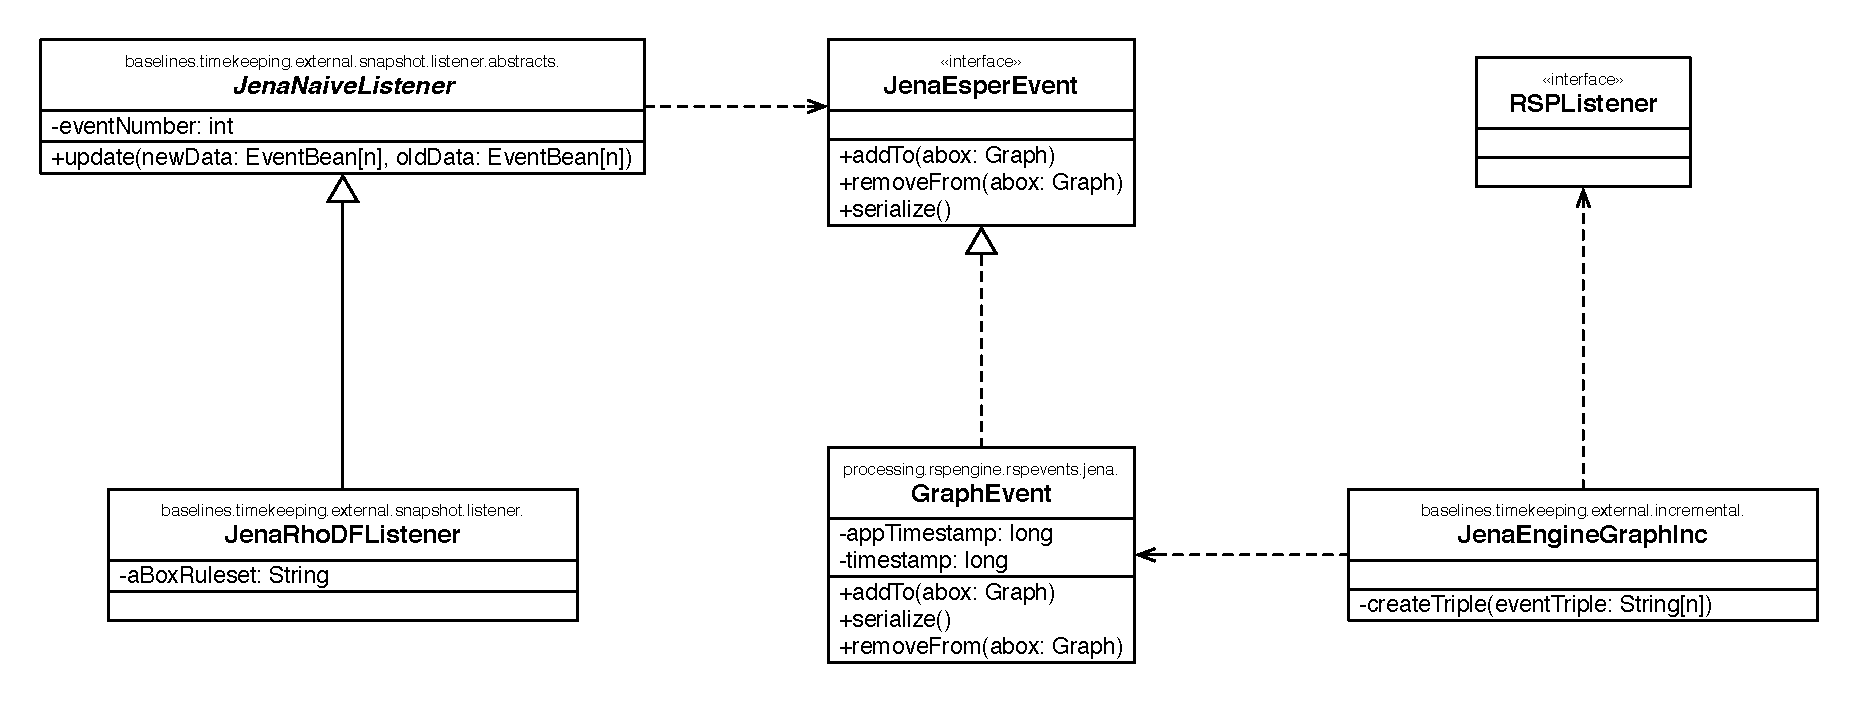
\includegraphics[width=\linewidth]{images/uml_baselines_rel_listener_event}
%	\caption[The Relation between \textit{RSPListener} and \textit{JenaEsperEvent} - UML Schema]{The listener and the event implementation are fully decoupled but logically related. In picture is detailed this relation for different implementation of the \textit{RSPListener}}
%  	\label{fig:uml_baselines_rel_listener_event}
%\end{figure}
%
%\textit{\textit{JenaNaiveListener} and the  \textit{JenaIncrementalListener} handle the events which come form the DSMS trough the \textit{JenaEsperEvent} interface, Figure~\ref{fig:uml_baselines_rel_listener_event} report  the structure for the case of Graph-based event representation (see Section~\ref{sec:baselines} for event details). }

\pagebreak

\section{Analyser}\label{sec:analyser-impl}

\begin{figure}[tbh]
  \centering
	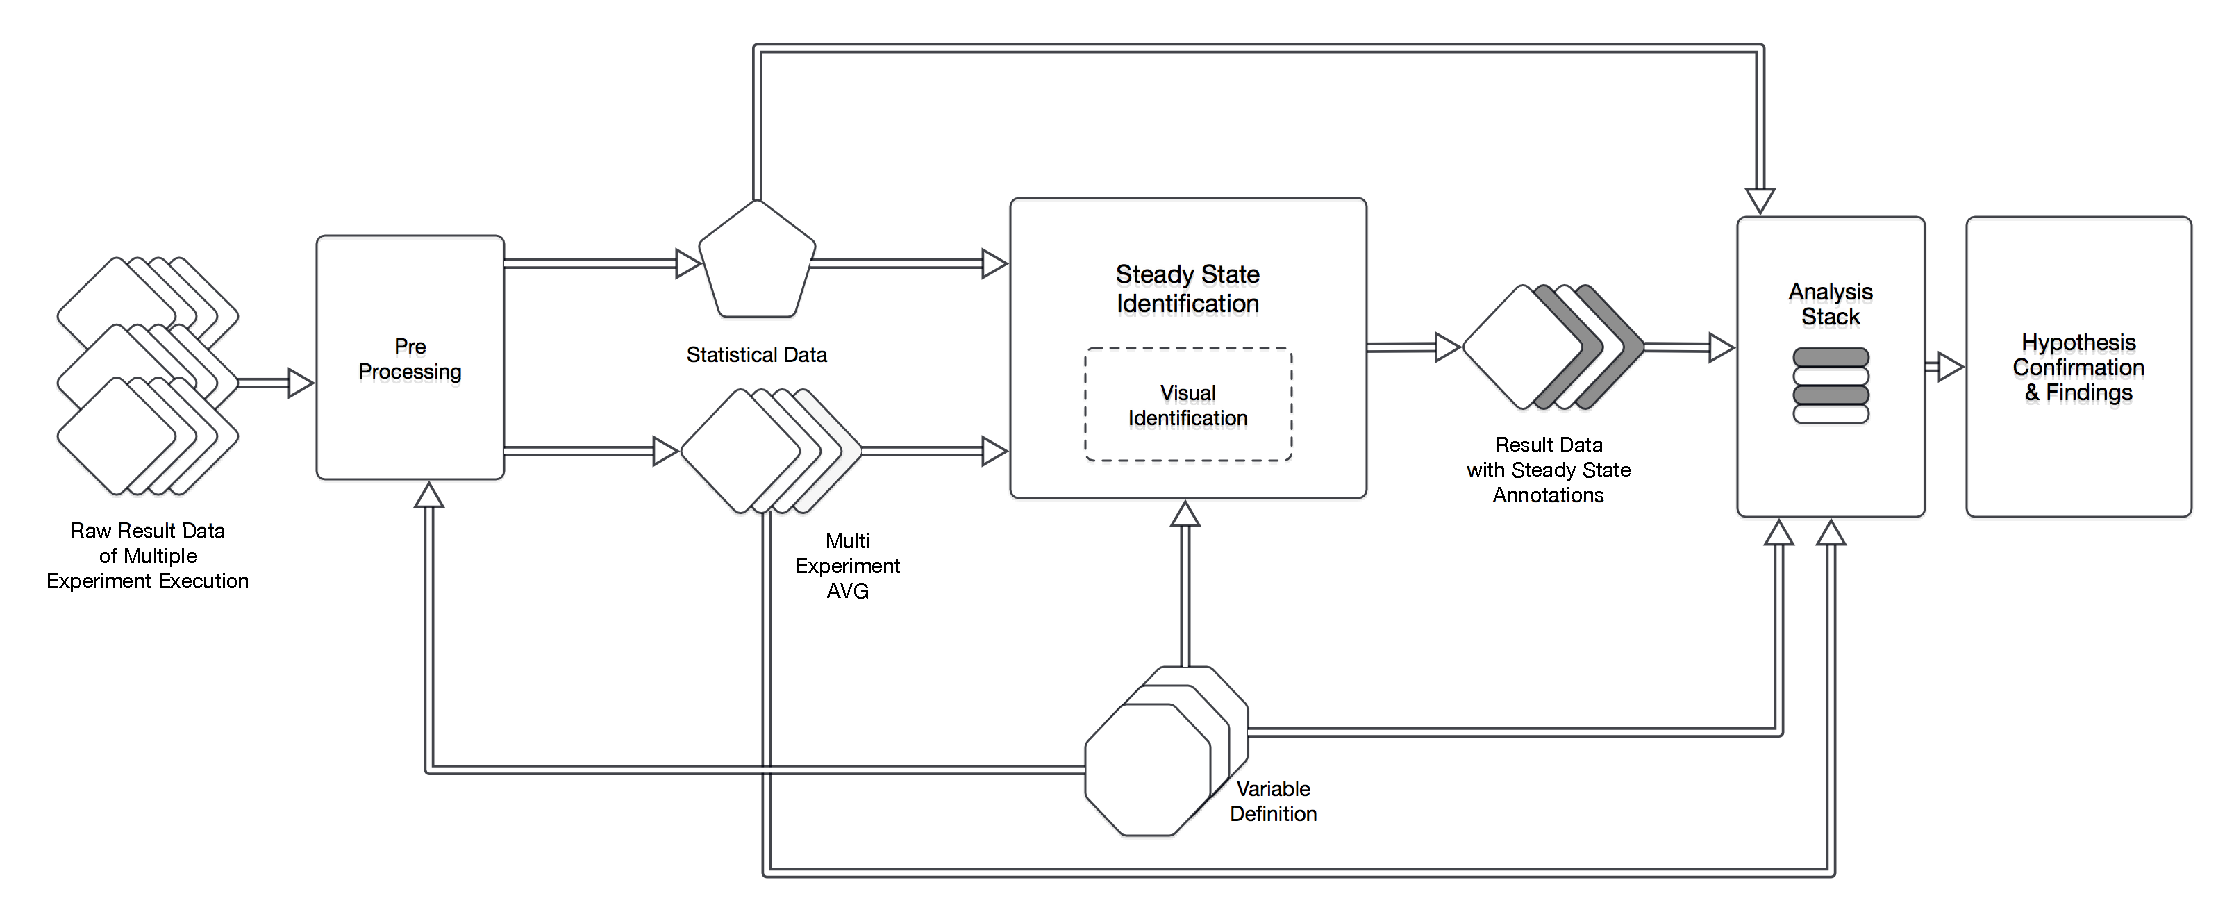
\includegraphics[width=\linewidth]{images/analyser-block-schema-impl}
	\caption[\textsc{Analyser} Block Schema: Implementation Detail Level]{The \textsc{Analyser} Block Schema in figure extends to the implementation detail the one of Figure~\ref{fig:analyser-block-schema}. Differently from the previous schema, a new initial block, name Pre-Processing, operates on the experiment raw data in two ways: it averages among multiple execution of the same experiment, to obtain a single reliable dataset for each experiment; it calculates statistical relevant values for each experiment (maximum, minimum, median ecc). This module receives as input also the involved variables to design pre-processing, while its outputs are consumed by the following modules as the figure shows.}
  	\label{fig:analyser-block-schema-impl}
\end{figure}

\noindent In this section we introduce which analysis tools sustain the each level in the investigation stack described in Section~\ref{sec:analyser} and how their realized in the current implementation of \name. Notice that the relation between the hypothesis and the tools that sustain the analysis is deep, thus it is hard to generalise the investigation toolset. Hypothesis depends on the the research question, while the tools are related to the nature of the data, which again concern the experiment.  However, there are some general meaningful characteristics, which are independent from both the hypothesis and experiment, that allow us to develop a basic toolset which sustains the entire investigation stack presented in Section~\ref{sec:analyser}.

Figure~\ref{fig:analyser-block-schema-impl} shows the different phases of data processing. It refers to the original block schema of drawn in Chapter~\ref{chap:heaven}, but Figure~\ref{fig:analyser-block-schema-impl} goes beyond the design level, providing some implementation details. 

The Figure~\ref{fig:analyser-block-schema-impl} shows the \textsc{Analyser} receives two input:
\begin{itemize}
\item the raw data form the experiments
\item the variables to build the analysis
\end{itemize}


In the original block schema (See Figure~\ref{fig:analyser-block-schema}) both inputs directly enter the \textit{Steady State Identification} Block (SSI) and the \textit{Analysis} Block (AB). In Figure~\ref{fig:analyser-block-schema-impl}   instead, the first block in the process is the \textit{Pre-Processing Block}. Empirical analysis can not rely on a single execution of an experiment, because even if the \textit{Test Stand} is designed to be system independent, it remains a dynamic system. Thus, strange behaviours may happen while an experiment is running. In order to reduce and possible eliminate the outliers, multiple runs of the same experiment must be mediated obtaining the average measures The \textit{Pre-Processing} Block ensures data reliability extrapolating a unique dataset from multiple executions. Moreover, time series describes how a dynamic system evolves over time, so it is meaningful to attempt hypothesis verification trough statistical values, which always consider the the Steady State to allow the generalisation of the insights. The \textit{Pre-Processing} Block calculates most common statistical metrics as average , standard deviation and maximum or minimum for a certain variable.

%Indeed, both the Steady State Identification Block and Analysis Block require an automatic procedure, named pre-processing in Figure~\ref{fig:analyser-block-schema-impl}, which averages the data of multiple executions of the same experiment and calculate the statistically relevant data. 

Once we have reliable data, the \textit{Steady State Identification} Block and the \textit{Analysis} Block receive them and start the analysis process. 

Finally, researches can read the analysis point out insight and theoretical results as the last block in the process describes.

Data mining procedures are very system-dependent. For this reason we include in Chapter~\ref{chap:evaluation} about the \name Evaluation, concrete analysis examples, by testing the Baselines. The aim of Chapter~\ref{chap:evaluation} is to demonstrate the value of \namens, but also we want to provide some guidelines for further evaluations.

The following subsections contains further details about the \textit{Steady State Identification} Block implementation, Subsection~\ref{sec:analyser-impl-ss-block}, and about the \textit{Analyser} Block with the investigation stack, Subsection~\ref{sec:analyser-impl-analysis-block}.

\subsection{Steady State Identification Block}\label{sec:analyser-impl-ss-block}

The Steady State Identification Block has the aim to  determines if a solution has reached the Steady State condition for a certain variable, as we describe in Section~\ref{sec:analyser-analysis-block}. Automatic procedures to identify the State State condition exist, but they require dedicated studies which will be faced as future works. Currently, the SSI is not automated. It exploits data visualisation techniques, to identify, if and when Steady State condition is reached. Practically each variable in the system is plotted in the time domain over all the entire experiment and research can exclude  the initial warm-up phase form the data evaluation when that variables reaches a stable condition. 
We know that the graphical method is limited, because it must be applied for each system variable, and human criteria can nit be reliable in this kind of analysis as automatic procedures which exploits tested algorithms. Moreover, different variables may reach the equilibrium at different times, so it is researcher responsibility to properly identify the different condition for each variable involved.

\subsection{Analysis Block}\label{sec:analyser-impl-analysis-block}

\noindent The \textsc{Analyser} Design includes Five Analysis Levels (see Section~\ref{sec:analyser} with increasing degrees of detail. The \textit{Analysis} Block hides the level where the comparative research approach is declined either to the visual analysis or statistical investigation. The graphical analysis method is more qualitative then the second one, but reading the information presented in graphical way can be preferred in those case where numerical data are not clear. On the other hand, the statistical investigation method demands more complex instruments to obtain the data, but allows to answer also elaborate questions with simpler answers. Following we present for all the Analysis level the method involved in the current implementation.

\subsubsection{Level 0 - Dashboards}\label{sec:impl-level0}

\begin{figure}[h!tbp]
  \centering
	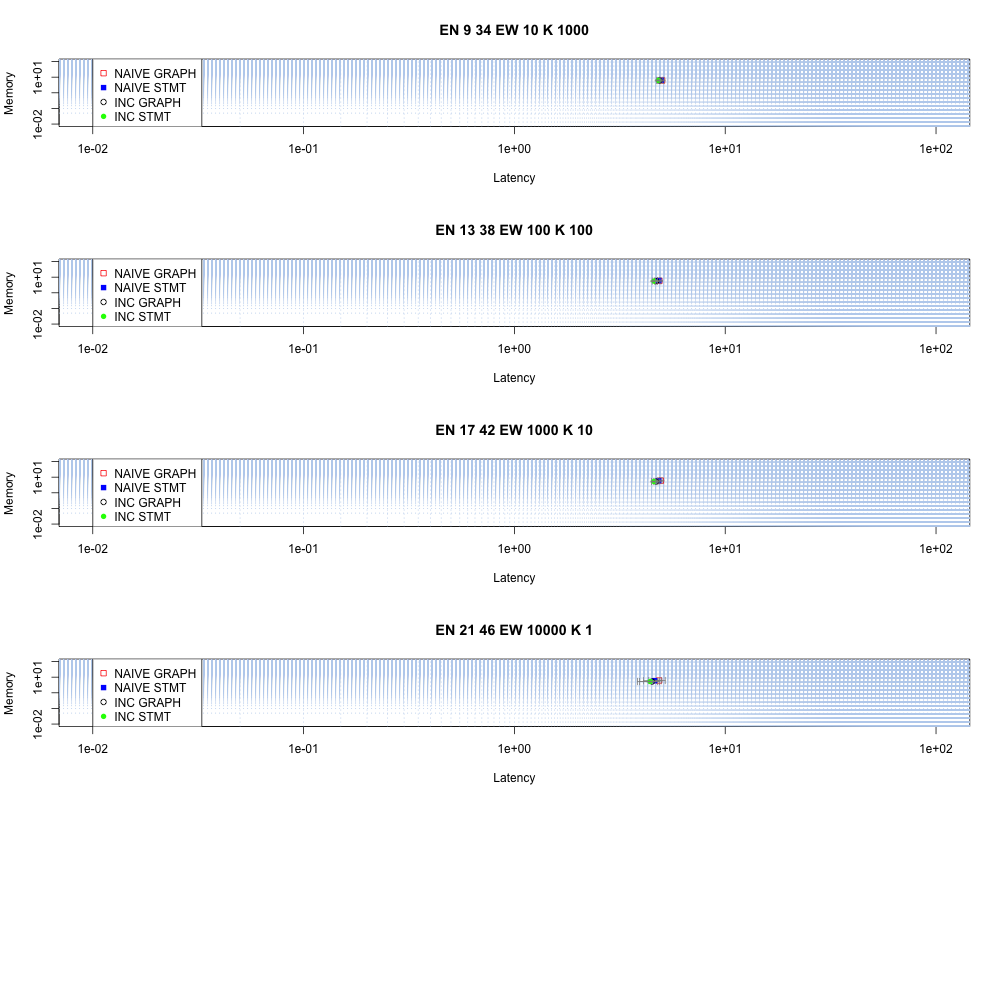
\includegraphics[width=0.45\linewidth]{images/dashboard-example}
	\caption[\textsc{Analyser} Investigation Stack - Level 0 -  Dashboard Representation Examples]{\textsc{Analyser} Investigation Stack - Level 0 -  Dashboard Representation Examples}
  	\label{fig:dashboard-example}
\end{figure}

\noindent Figure~\ref{fig:dashboard-example} contains an example of the possible Dashboard representations. We implement the dashboard to represent data on a bi-dimensional Cartesian space where memory and latency are the axis of the graph. This kind of representation allows to define solution dominance, w.r.t the involved variable, trough inter-experiment comparisons. Thus, we can easily state which RSP Engine, if any, is better then another one looking to a dashboard.

\subsubsection{Level 1 - Statistical Values Comparison}\label{sec:impl-level1}

Tables~\ref{tab:comp-tables} (a) and (b) show two examples of statistical investigation. Table~\ref{tab:comp-tables}.a contains the qualitative comparison of two solution over a given variable, while Table~\ref{tab:comp-tables}.b offers a deeper details level, the quantitative comparison, showing how much a solution is better than the other. How to choose the proper level depends on the needs of the research.

\begin{table}[htb]
\scriptsize
	\centering
	\subtable[Symbolic Comparison of variables A vs B on Experiment 1]{%
		\begin{tabular}{c | cccc} % creating eight columns
	  	\hline
		A vs B & \multicolumn{4}{c}{Experiment 1 Condition A}  \\
		 Comparison  & &&&\\
		\hline
		   	        & $\simeq$\\
		 Experiment 1 & A     & 	$\simeq$  & A & B\\
		 Condition  & A     & 	$\simeq$  & $\simeq$ & B\\
		 B          & A     & 	$\simeq$  & B & A\\
		\hline % inserts single-line
	 \end{tabular}
	}\qquad\qquad
	\subtable[Symbolic Comparison of variables A vs B on Experiment 1]{%
		\begin{tabular}{c | cccc} % creating eight columns
	  	\hline
		A vs B & \multicolumn{4}{c}{Experiment 1 Condition A}  \\
		 Comparison  & &&&\\
		\hline
		   	        & $\simeq$\\
		 Experiment 1 & 10\%     & 	$\simeq$  & 42\% & 33\%\\
		 Condition  & 23\%     & 	$\simeq$  & $\simeq$ & 12\%\\
		 B          & 20\%    & 	$\simeq$  & 22\% & 22\%\\
		\hline % inserts single-line
	 \end{tabular}
	}
	\caption[\textsc{Analyser} Investigation Stack - Level 1 - Qualitative and Quantitative Comparison Examples]{\textsc{Analyser} Investigation Stack - Level 1 - Example of qualitative-comparison over two variables  (a)  and  quantitative-comparison over a common variable (b) }
	\label{tab:comp-tables}
\end{table}

Table layout is a key-point for Level 1 representations. Tables axes represent the variation of two different experiment properties A and B. Different experiments influence the behaviour of an RSP Engine in different ways, and Level 1 allows to point out this differences with  \textit{Inter-Experiment} comparisons. Thus, we can move on the horizontal axis of Table~\ref{tab:comp-tables}.a, which means variate the Condition A, to appreciate those differences. 

Actually this kind of analysis is possible thanks to a CSV report, which contains all the meaningful statistical values for the experiments. The report can be further manipulated to obtain the table visualisation.

\subsubsection{Level 2 - Patter Identification}\label{sec:impl-level2}

%\begin{figure}[tbh]
%  \centering
%   \subfigure[Pattern Recognition Example: Memory in Time Domain]{
%  	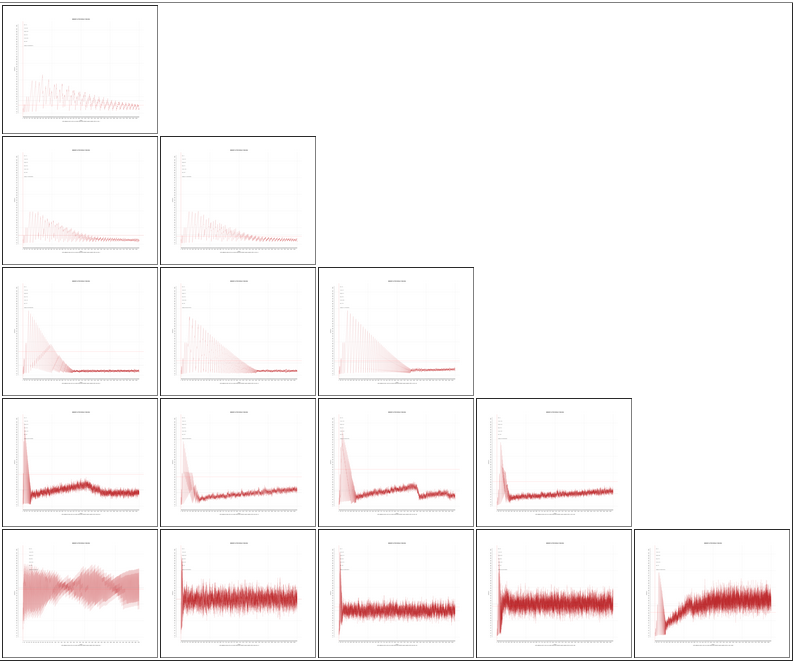
\includegraphics[width=0.45\linewidth]{images/pattern-example-memory}
%  }
%  \subfigure[Pattern Recognition Example: Memory Distribution]{
%  	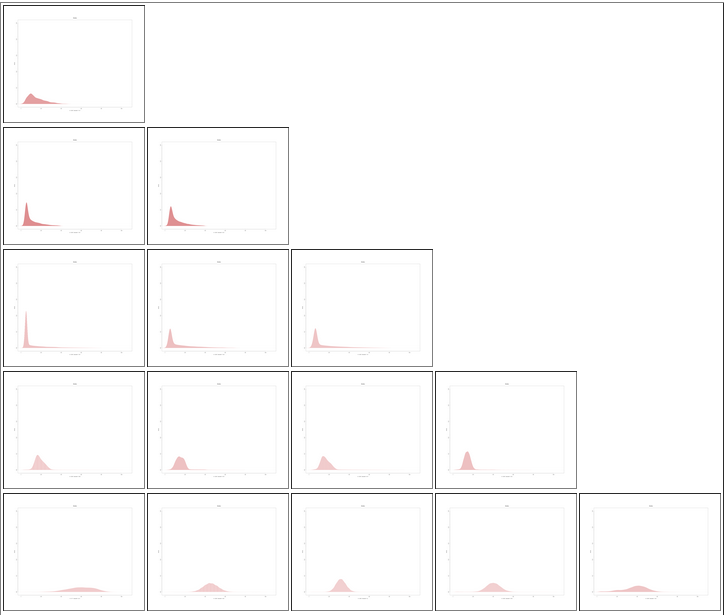
\includegraphics[width=0.45\linewidth]{images/pattern-example-density}
%  	
%  }
%   %\subfigure[Pattern Appear On the Wall..]{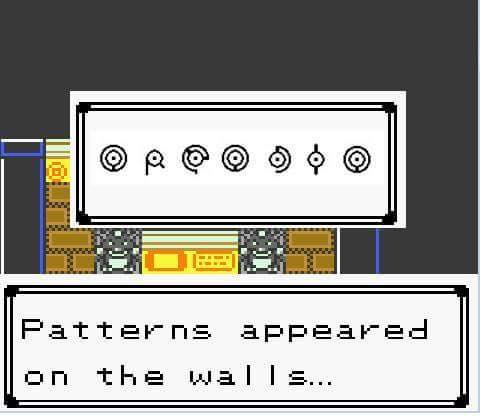
\includegraphics[width=0.45\linewidth]{images/pokepattern}}
%	\caption[\textsc{Analyser} Investigation Stack - Level 2 - Pattern Recognition Examples]{Two examples of pattern recognition. Level 2 exploits  easy-to-read layouts which highlights the experiment difference to enable \textit{Inter Experiment} comparisons} 
%  	\label{fig:pattern-examples}
%\end{figure}

\begin{table}[htbp]
	\centering
	\scriptsize
	\subtable[Pattern Recognition Example: Memory Time Domain]{%
		\begin{tabular}{l | ccccc} % creating eight columns
	  	\hline
		Triple  & \multicolumn{5}{c}{Slots}  \\
		in & \multicolumn{5}{c}{Number}  \\
		Window  & 1 & 10 & 100 & 1000&10000\\
		\hline
		1	   &\begin{minipage}{.1\textwidth}
     			 	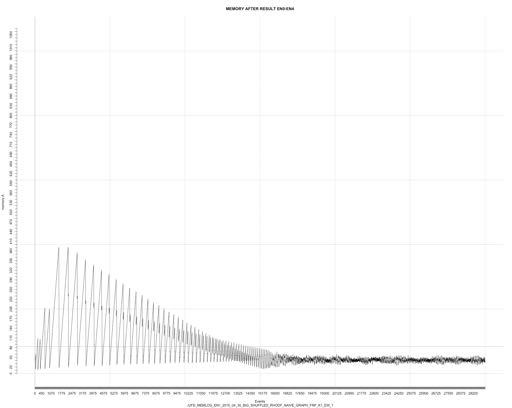
\includegraphics[width=\linewidth]{images/mema-graph/N1}
    				 \end{minipage}\\			
		10	   & \begin{minipage}{.1\textwidth}
     			 	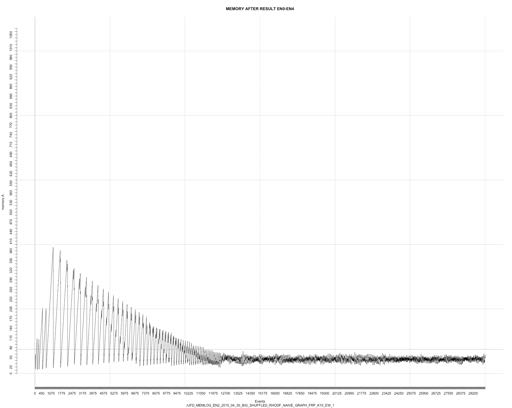
\includegraphics[width=\linewidth]{images/mema-graph/N2}
    				\end{minipage}
    			   & \begin{minipage}{.1\textwidth}
     			 	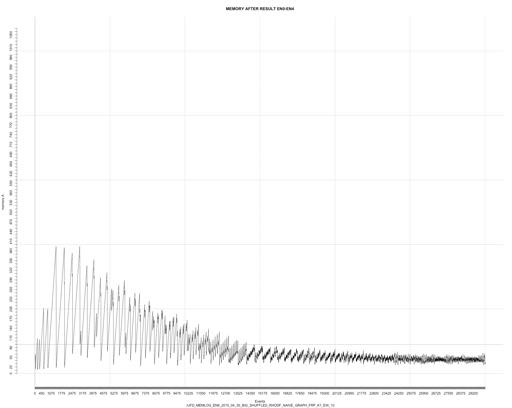
\includegraphics[width=\linewidth]{images/mema-graph/N6}
    				 \end{minipage}\\		
		100	   & \begin{minipage}{.1\textwidth}
     			 	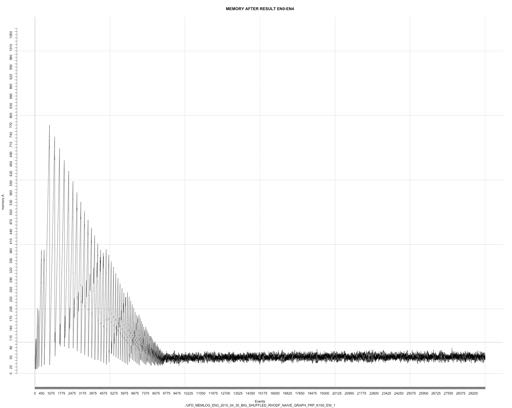
\includegraphics[width=\linewidth]{images/mema-graph/N3}
    				 \end{minipage}
    			   & \begin{minipage}{.1\textwidth}
     			 	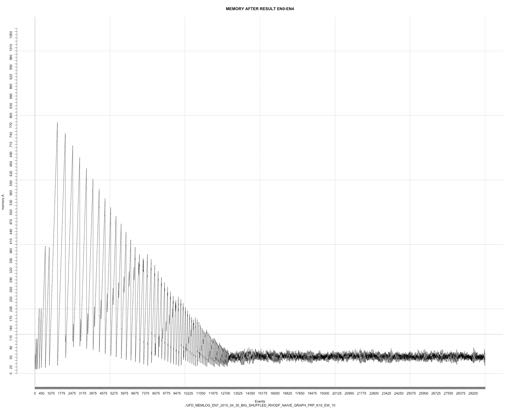
\includegraphics[width=\linewidth]{images/mema-graph/N7}
    				 \end{minipage}
    			   &	 \begin{minipage}{.1\textwidth}
     			 	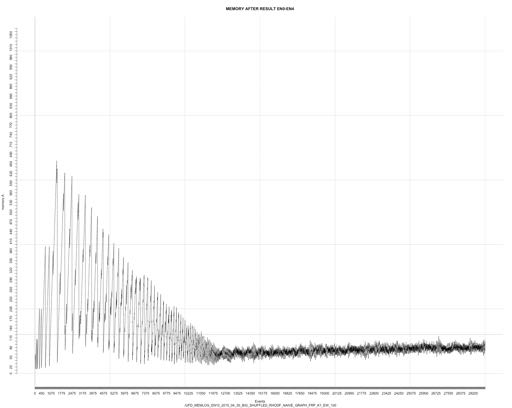
\includegraphics[width=\linewidth]{images/mema-graph/N10}
    				 \end{minipage}\\	
		1000   &	 \begin{minipage}{.1\textwidth}
     			 	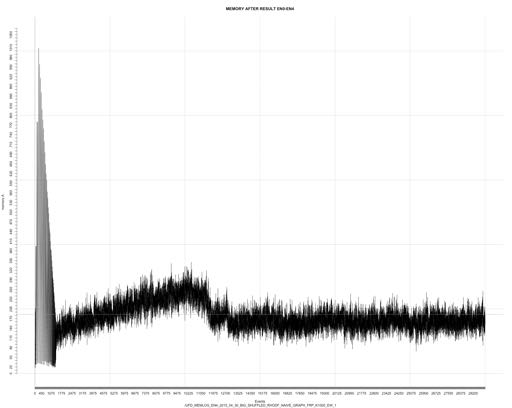
\includegraphics[width=\linewidth]{images/mema-graph/N4}
    				 \end{minipage}
    			   &	 \begin{minipage}{.1\textwidth}
     			 	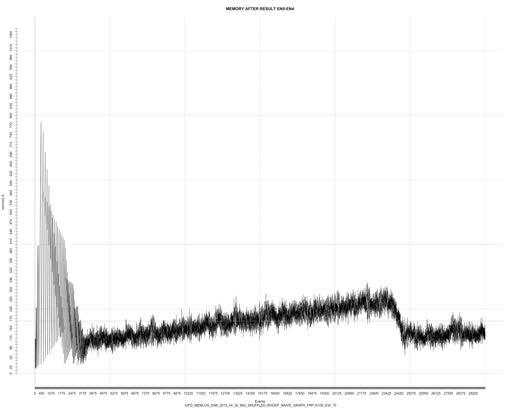
\includegraphics[width=\linewidth]{images/mema-graph/N8}
    				 \end{minipage}
    			   &	 \begin{minipage}{.1\textwidth}
     			 	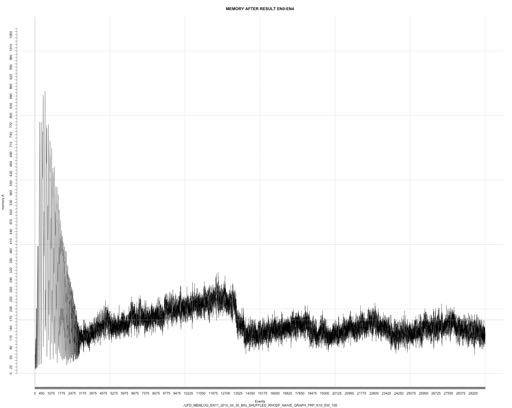
\includegraphics[width=\linewidth]{images/mema-graph/N11}
    				 \end{minipage}
    			   &	 \begin{minipage}{.1\textwidth}
     			 	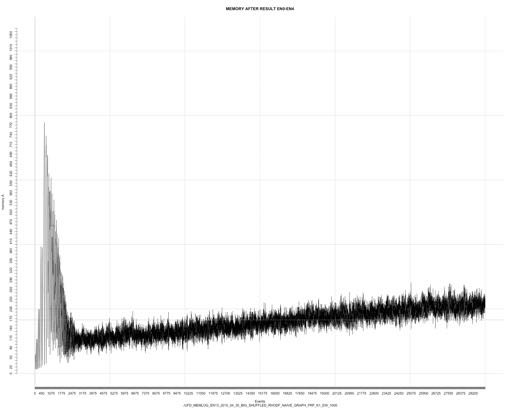
\includegraphics[width=\linewidth]{images/mema-graph/N13}
    				 \end{minipage}\\
		10000  &	 \begin{minipage}{.1\textwidth}
     			 	
\includegraphics[width=\linewidth]{images/mema-graph/N5}
    				 \end{minipage}
    			   &	 \begin{minipage}{.1\textwidth}
     			 	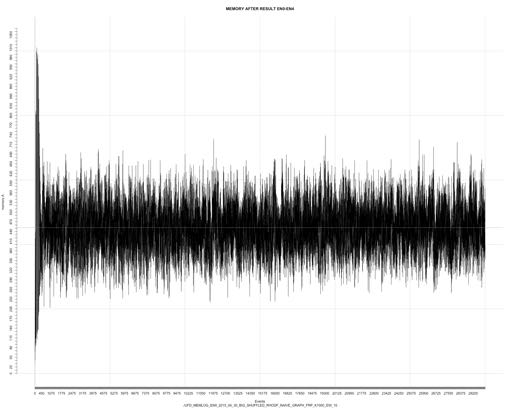
\includegraphics[width=\linewidth]{images/mema-graph/N9}
    				 \end{minipage}
    			   &	 \begin{minipage}{.1\textwidth}
     			 	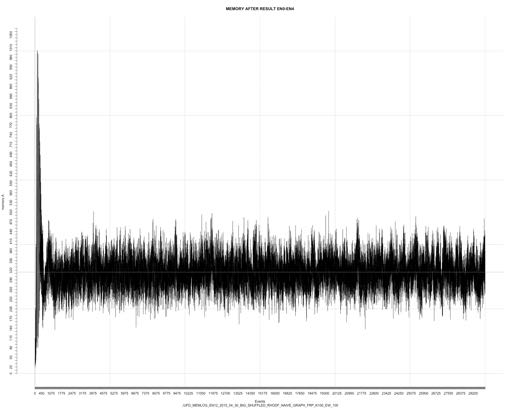
\includegraphics[width=\linewidth]{images/mema-graph/N12}
    				 \end{minipage}
    			   &	 \begin{minipage}{.1\textwidth}
     			 	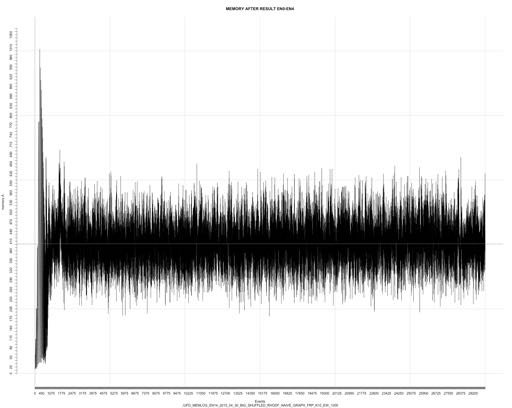
\includegraphics[width=\linewidth]{images/mema-graph/N14}
    				 \end{minipage}
    			   &	 \begin{minipage}{.1\textwidth}
     			 	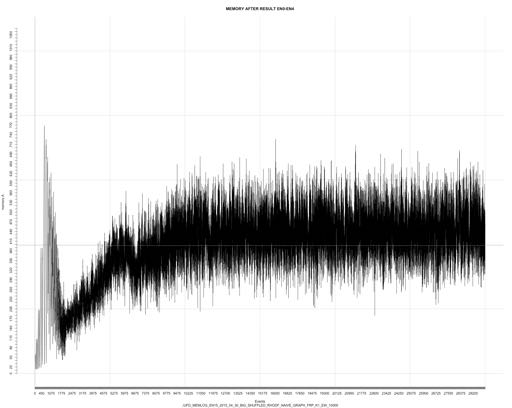
\includegraphics[width=\linewidth]{images/mema-graph/N15}
    				 \end{minipage}\\
		\hline % inserts single-line
	 \end{tabular}
	}
	\subtable[Pattern Recognition Example: Memory Distribution]{%
		\begin{tabular}{l | ccccc} % creating eight columns
	  	\hline
		Triple  & \multicolumn{5}{c}{Slots}  \\
		in & \multicolumn{5}{c}{Number}  \\
		Window  & 1 & 10 & 100 & 1000&10000\\
		\hline
		1	   &\begin{minipage}{.1\textwidth}
     			 	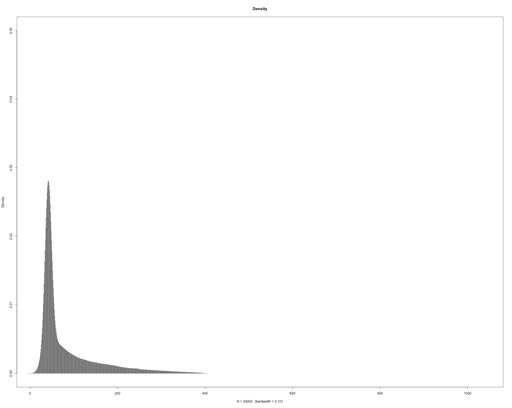
\includegraphics[width=\linewidth]{images/mema-dens-graph/N1}
    				 \end{minipage}\\			
		10	   & \begin{minipage}{.1\textwidth}
     			 	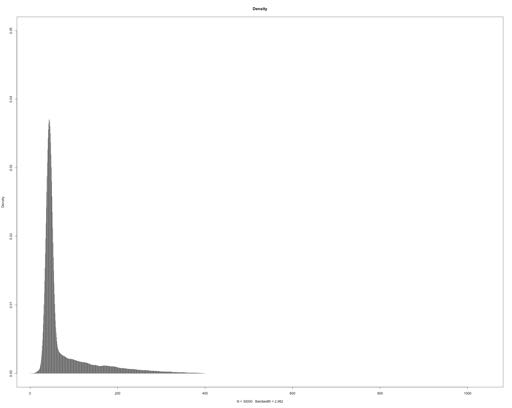
\includegraphics[width=\linewidth]{images/mema-dens-graph/N2}
    				\end{minipage}
    			   & \begin{minipage}{.1\textwidth}
     			 	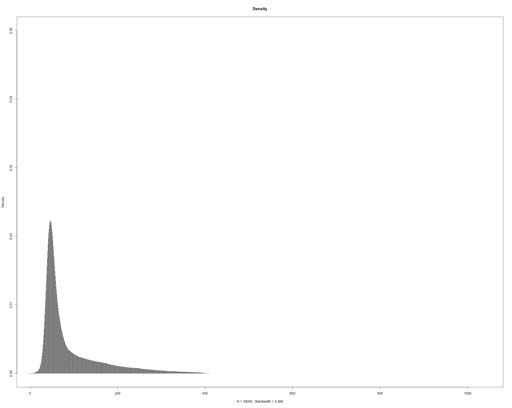
\includegraphics[width=\linewidth]{images/mema-dens-graph/N6}
    				 \end{minipage}\\		
		100	   & \begin{minipage}{.1\textwidth}
     			 	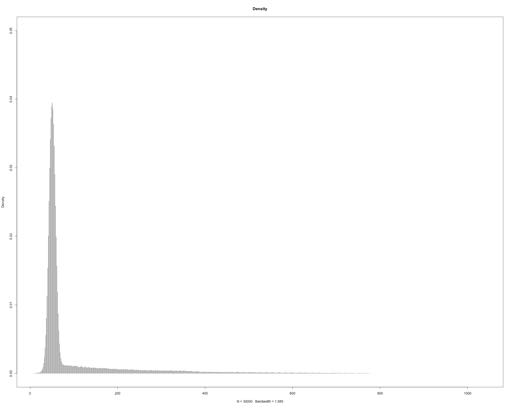
\includegraphics[width=\linewidth]{images/mema-dens-graph/N3}
    				 \end{minipage}
    			   & \begin{minipage}{.1\textwidth}
     			 	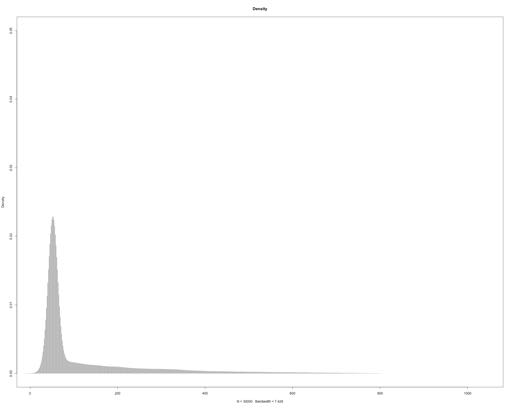
\includegraphics[width=\linewidth]{images/mema-dens-graph/N7}
    				 \end{minipage}
    			   &	 \begin{minipage}{.1\textwidth}
     			 	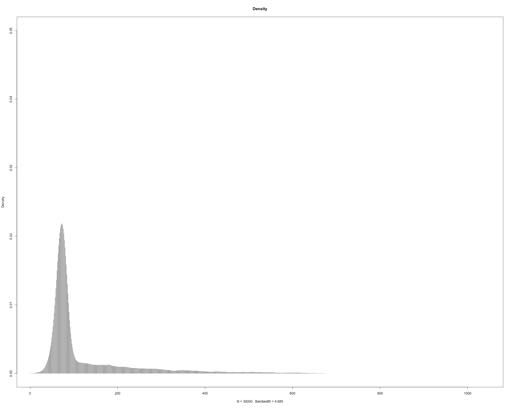
\includegraphics[width=\linewidth]{images/mema-dens-graph/N10}
    				 \end{minipage}\\	
		1000   &	 \begin{minipage}{.1\textwidth}
     			 	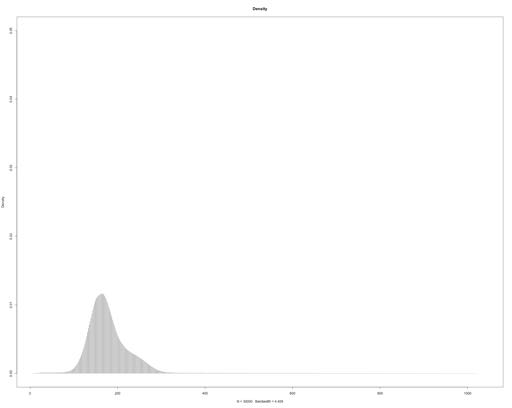
\includegraphics[width=\linewidth]{images/mema-dens-graph/N4}
    				 \end{minipage}
    			   &	 \begin{minipage}{.1\textwidth}
     			 	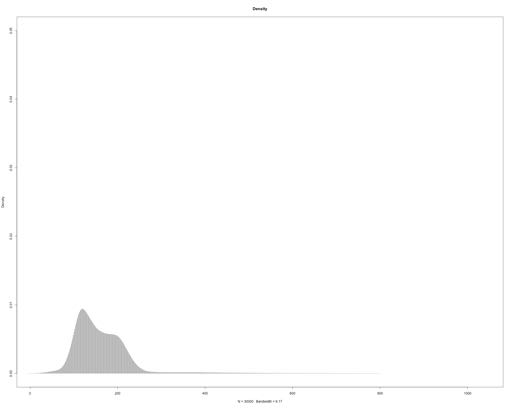
\includegraphics[width=\linewidth]{images/mema-dens-graph/N8}
    				 \end{minipage}
    			   &	 \begin{minipage}{.1\textwidth}
     			 	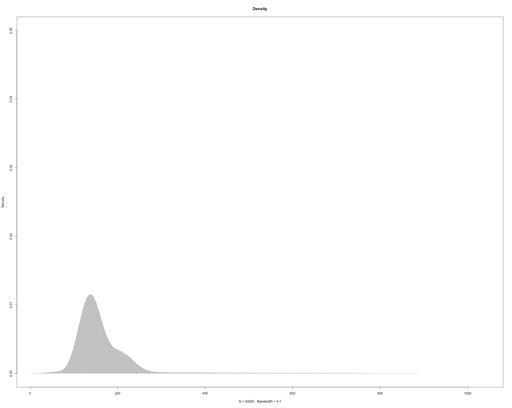
\includegraphics[width=\linewidth]{images/mema-dens-graph/N11}
    				 \end{minipage}
    			   &	 \begin{minipage}{.1\textwidth}
     			 	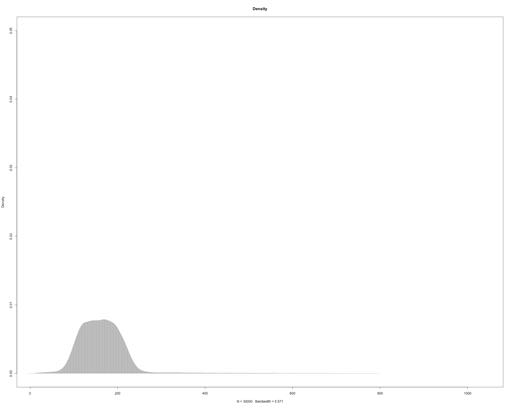
\includegraphics[width=\linewidth]{images/mema-dens-graph/N13}
    				 \end{minipage}\\
		10000  &	 \begin{minipage}{.1\textwidth}
     			 	
\includegraphics[width=\linewidth]{images/mema-dens-graph/N5}
    				 \end{minipage}
    			   &	 \begin{minipage}{.1\textwidth}
     			 	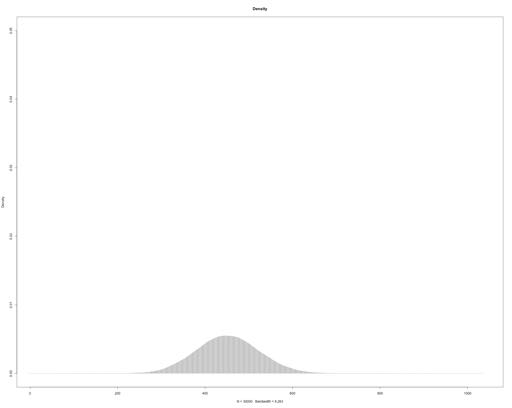
\includegraphics[width=\linewidth]{images/mema-dens-graph/N9}
    				 \end{minipage}
    			   &	 \begin{minipage}{.1\textwidth}
     			 	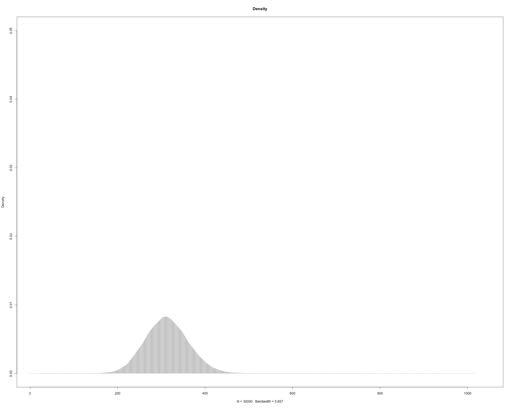
\includegraphics[width=\linewidth]{images/mema-dens-graph/N12}
    				 \end{minipage}
    			   &	 \begin{minipage}{.1\textwidth}
     			 	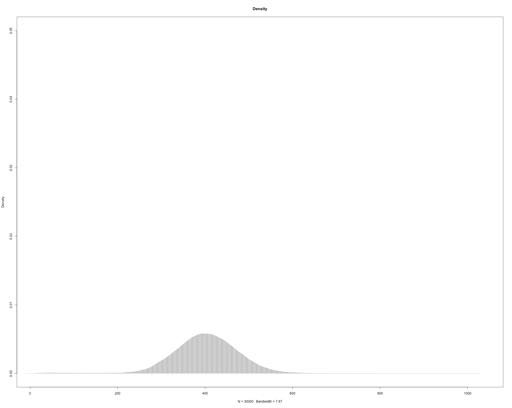
\includegraphics[width=\linewidth]{images/mema-dens-graph/N14}
    				 \end{minipage}
    			   &	 \begin{minipage}{.1\textwidth}
     			 	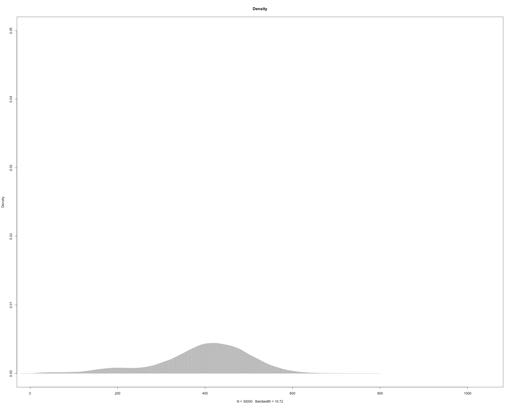
\includegraphics[width=\linewidth]{images/mema-dens-graph/N15}
    				 \end{minipage}\\
		\hline % inserts single-line
	 \end{tabular}
	}
	\caption[\textsc{Analyser} Investigation Stack - Level 2 - Pattern Recognition Examples]{Two examples of pattern recognition. Level 2 exploits  easy-to-read layouts which highlights the experiment difference to enable \textit{Inter Experiment} comparisons} 
	\label{tab:pattern-examples}	
\end{table}

\noindent Level 2 exploits the same experiment layout of Level 1 to compare many graphical representation of the experiment variable. Two examples of memory analysis at Level 2 are reported in Tables~\ref{tab:pattern-examples} (a) and (b). Table~\ref{tab:pattern-examples}.a show the memory behaviour in time domain. It allows answer questions like "How the system changes the memory behaviour changing the input dimension?". Table~\ref{tab:pattern-examples}.b reports the distribution memory values upon several intervals. It allows to understand how memory distribution is influenced by changing the variable on the Table axes or diagonals.

Level 3 aims of pattern identification for a given variable in an experimental set. It is an example of \textit{Inter-Experiment} comparison which enable a new kind of global analysis, because it requires to state observation upon the entire set of experiment.

\subsubsection{Level 3 - Visual Comparison}\label{sec:impl-level3}

\noindent Finally, Level 3 focuses on single graphical visualisation. Figure~\ref{fig:visual-comp} contains two examples of the possible analysis. Figure~\ref{fig:visual-comp}.a shows a case of \textit{Inter Experiment}comparison, highlighting the relation between the same variable over multiple experiments; Figure~\ref{fig:visual-comp}.b provides an example of \textit{Intra Experiment} comparison, highlighting the relation between memory and latency within the same experiment.

\begin{figure}[tbh]
  \centering
  \subfigure[Multi-Experiment Comparison]{
  			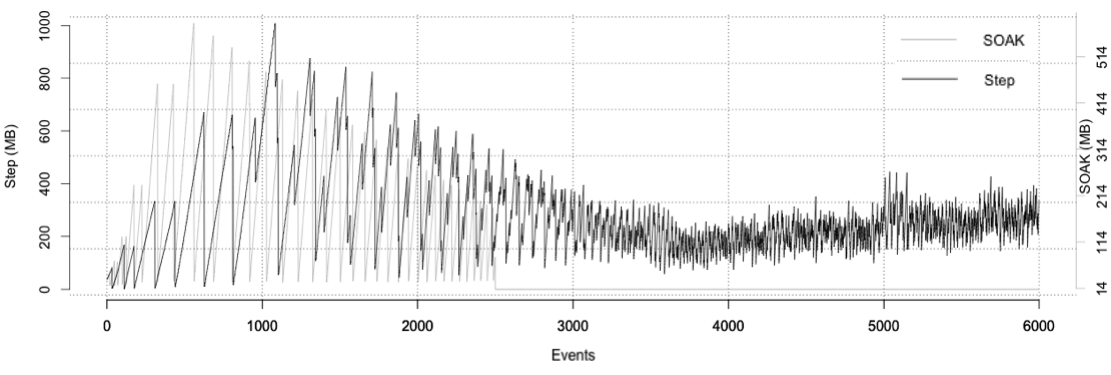
\includegraphics[width=0.70\linewidth]{images/comp-inter}
  			}
  \subfigure[Multi-Variables Comparison]{
  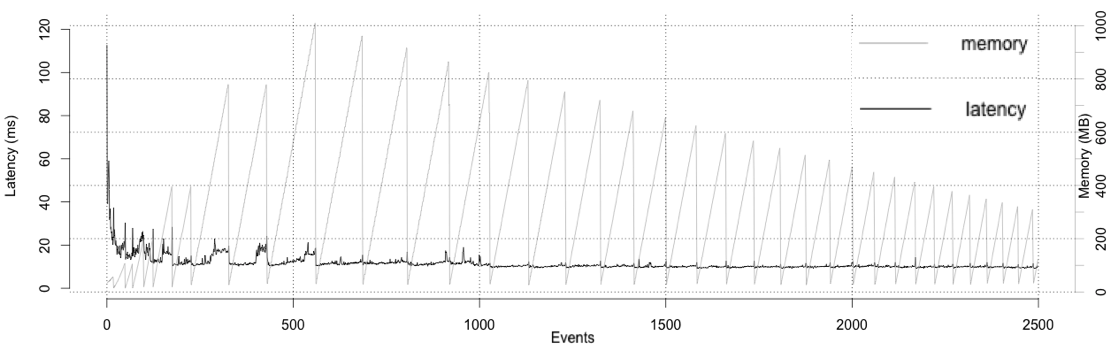
\includegraphics[width=0.70\linewidth]{images/comp-intra}
  }
\caption[\textsc{Analyser} Investigation Stack - Level 3 - Visual Comparison Examples]{\textsc{Analyser} Investigation Stack - Level 3 - Figure (a) shows a case of \textit{Inter Experiment} visual comparison of the memory usage while Figure (b) present a case of \textit{Intra Experiment} comparison of latency and memory.}
  \label{fig:visual-comp}
\end{figure}